\documentclass[a4paper]{article}
\usepackage{graphicx}
\usepackage{biblatex} %Imports biblatex package
\addbibresource{literature.bib} %Imports bibliography file
\usepackage{wrapfig}
\usepackage{geometry}
 \geometry{
 total={170mm,250mm},
 top=15mm,
 }
 \usepackage{blindtext}
% Load the setspace package
\usepackage{setspace}
\setstretch{1.5}
\setcounter{tocdepth}{4}
\setlength{\parindent}{0pt}
\usepackage{lipsum}
\usepackage{amssymb,amsmath}
\usepackage{siunitx}

\date{November 2024}


\begin{document}
\thispagestyle{empty}

\begin{figure}
    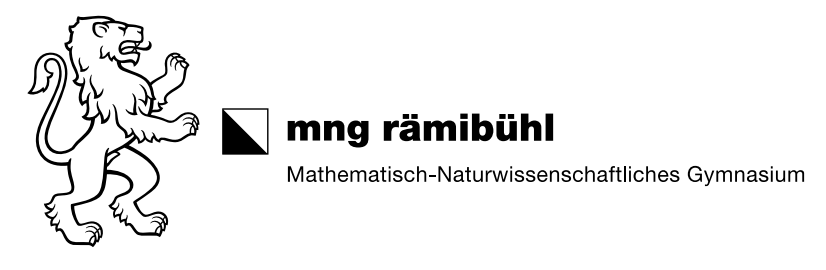
\includegraphics[width=0.4\textwidth]{images/MNG_pic.png}
\end{figure}
\begin{center}
    \large
    Irina Tiknonovskaia\\
    \Huge \textbf{Raman Spectroscopy}
    \\[0.5cm]
    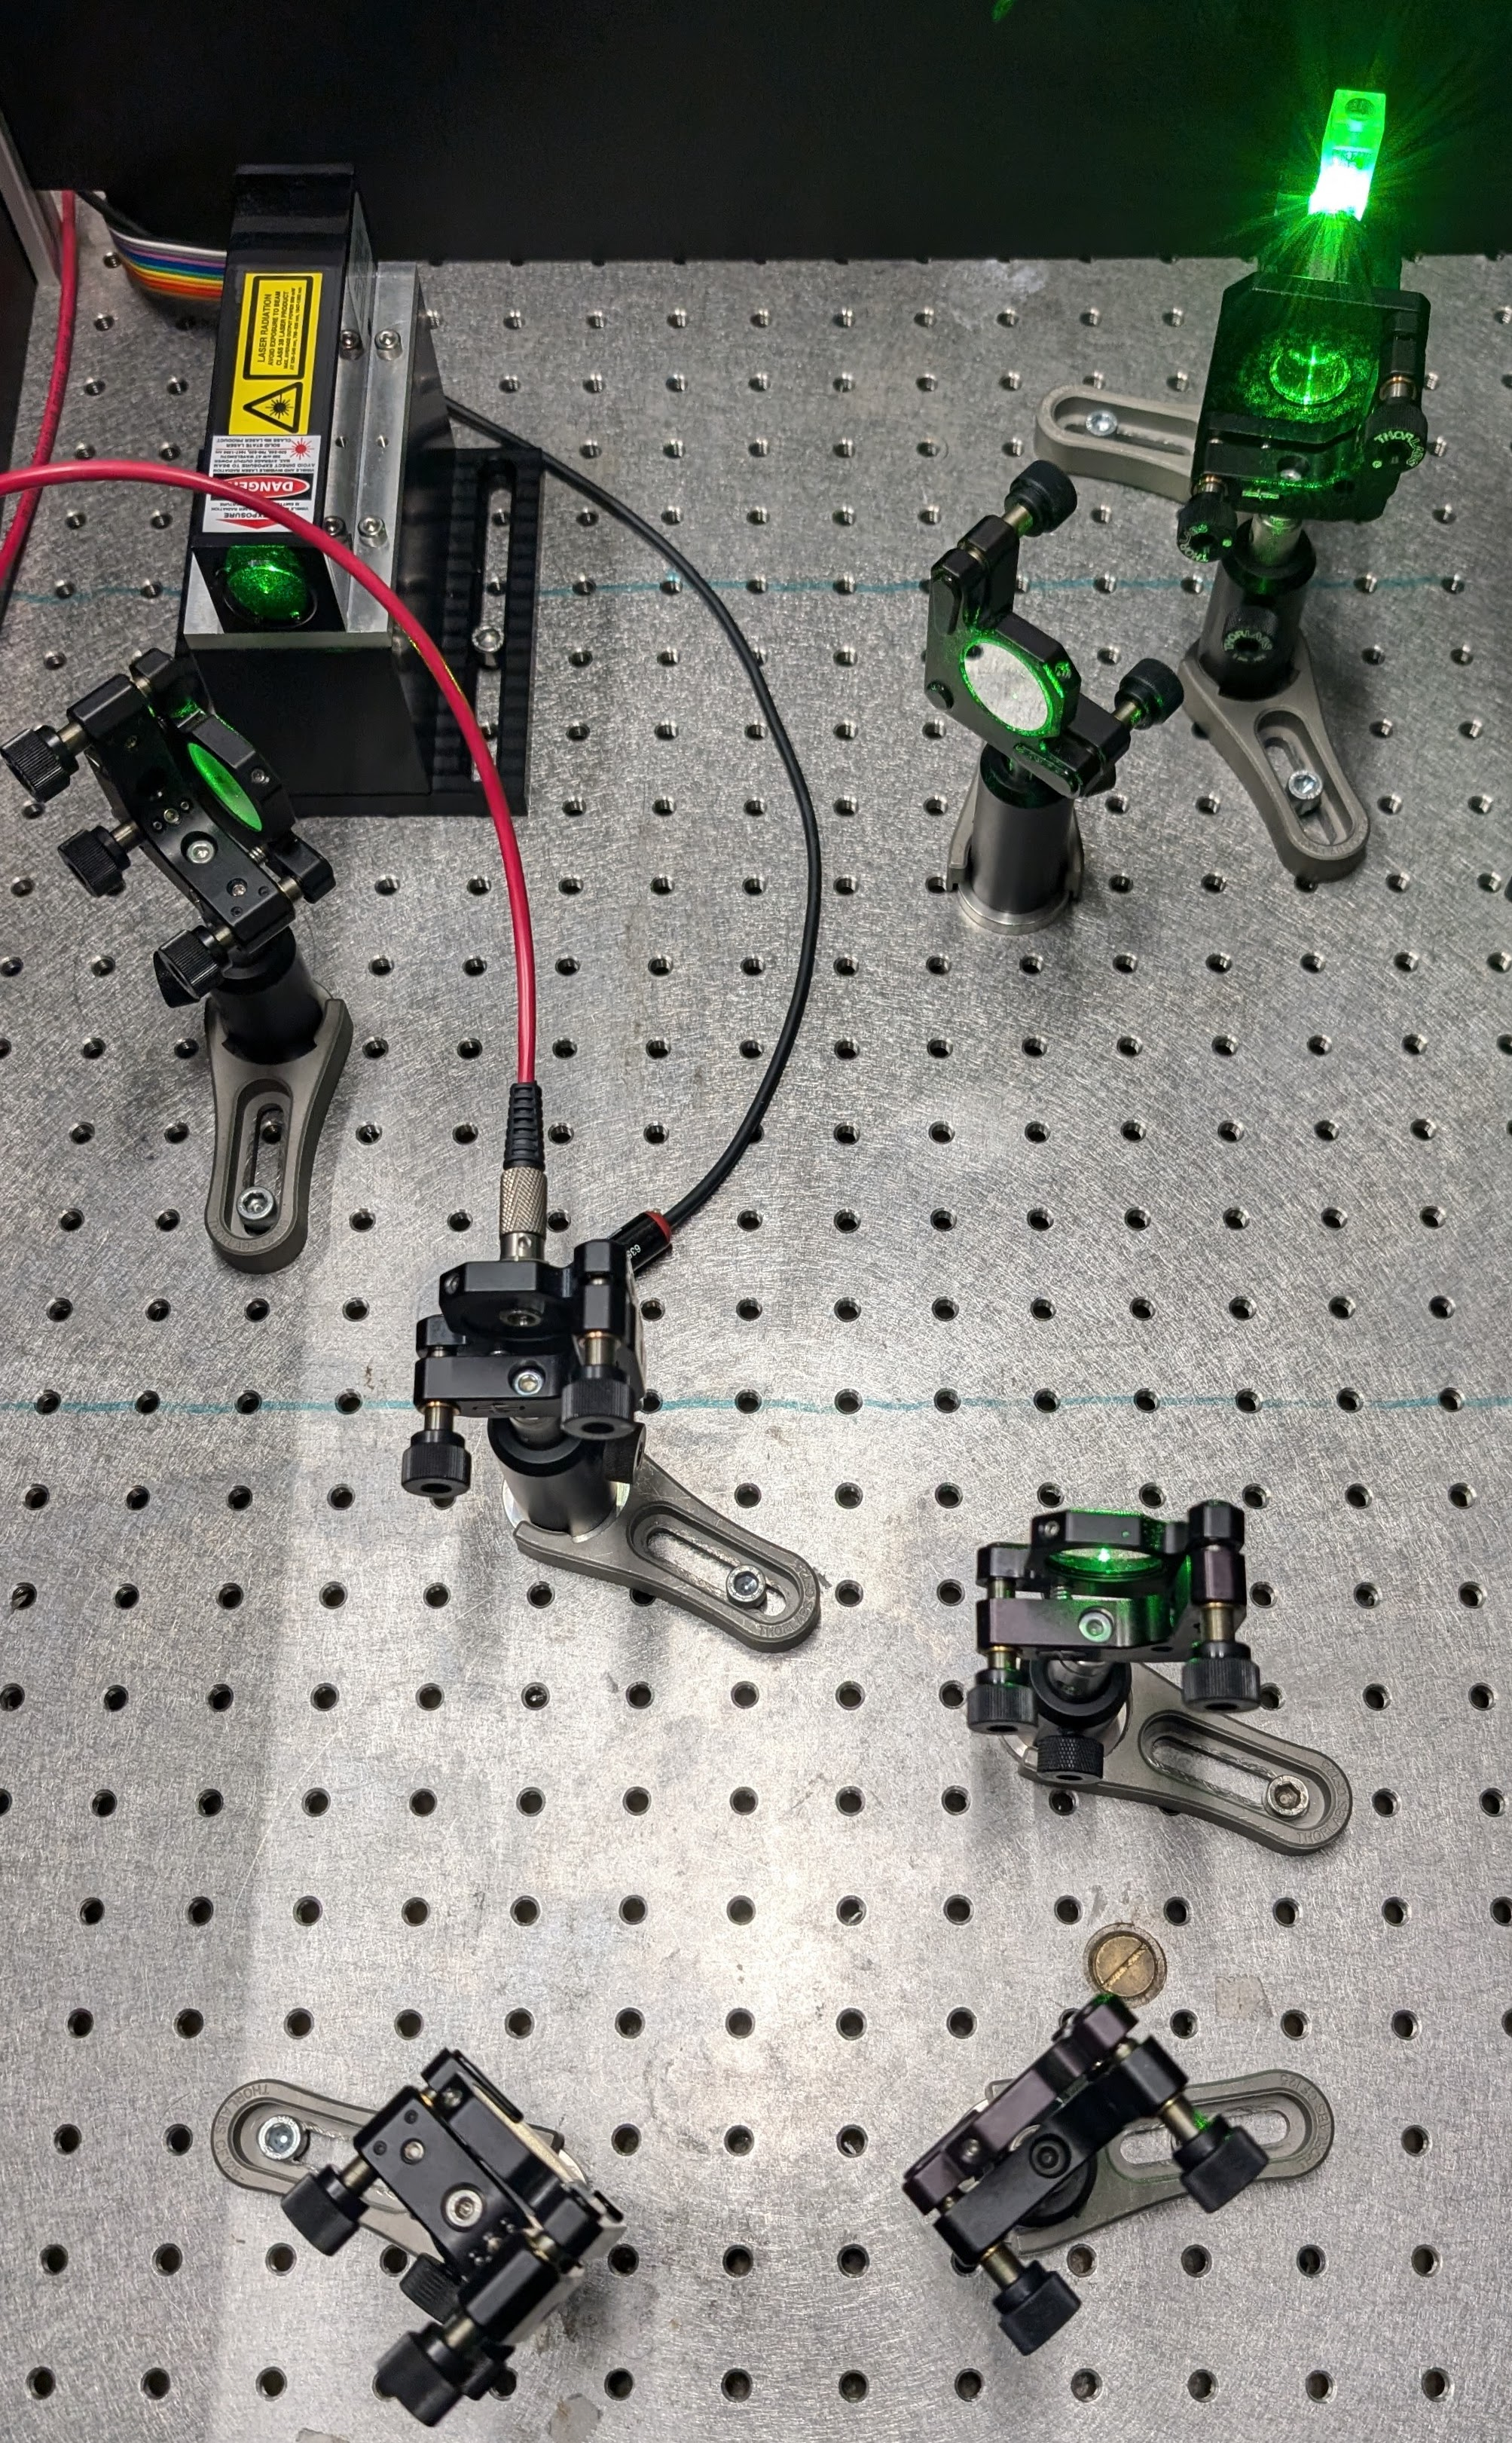
\includegraphics[width=9cm]{images/active_setup_photo.jpg}
    \\[0.5cm]
    \large
    \textbf{Matura Thesis}\\
    in the Subject Physics
    \\[0.25cm]
    \textbf{Supervision}\\
    Dipl. Phys. ETH Daniel Keller
    \\[0.25cm]
    6. January 2025
\end{center}
\newpage
\newgeometry{
 a4paper,
 total={140mm,230mm},
 top=30mm,
 }

\section*{Acknowledgements}

I would like to thank Prof. Dr. Frédéric Merkt for giving me the opportunitz to perform my experiments at ETH, and Maxime Holdener for taking the time to supervise me throughout the experiments, as well as establishing the first contact to Prof. Merkt. I would like to thank Daniel Keller for his dedicated support and supervision of this work. Especially for his assistance regarding the organisation of the experiment with ETH Zürich. Lastly, I would like to thank all other people who have supported me throughout this process, be it emotionally, when I asked stupid questions or when I asked then to proofread my writing.

\newpage


\section*{Abstract}

This thesis presents a study on Raman spectroscopy based on the 17th task statement of the International Young Physicists' Tournament (IYPT) 2025. It is a problem in the field of quantum mechanics, though it is also central in the field of physical chemistry. Changes in the wavelengths of scattered light are investigated. First the phenomenon of Raman scattering is qualitatively explained using a classical mechanics approach, and second, modified to explain a discreptancy between the Stokes and anti-Stokes shifts. To verify the theory, experiments were conducted, for the setup of which the needed materials and methods are discussed. The experimental data is evaluated and compared to literature values, very good agreement is achieved. The content of this thesis will be developed in preparation for the Swiss Young Physicists' Tournament (SYPT) and the International Young Physicists' Tournament (IYPT).

\newpage

\tableofcontents
\newpage

\section{History and Applications}
In 1928, a letter from the Indian physicist Chandrasekhara Venkata Raman, often referred to as C.V. Raman, and his student Kariamanikkam Srinivasa Krishnan, usually mentioned as K.S. Krishnan, was published in \textit{Nature}. This letter, named \textit{A New Type Of Secondary Radiation}, outlined their findings on the topic of modified scattered radiation, which is now referred to as Raman scattering. It was the result of several years of hard work and dedication from Raman and his students, of which Krishnan is the most well known, but not the only one. Afterwards, C.V. Raman published several papers on Raman scattering and spectroscopy. For his work, C.V. Raman has recieved a Nobel Prize in Physics. \cite{ram28}
\bigskip

While this was the first time that this phenomenon has been observed, it has been predicted theoretically in 1923 by the austrian physicist Adolf Smekal.
\bigskip

In the beginning, before the invention of lasers, the sun was used as a light source, with filters and lenses to focus it and to limit the wavelength, and with it the colour of the light. Using this setup and the existing spectrographs, very long integration times were needed in order to obtain measureable  spectra due to low sensitivity and the fact that Raman scattering is a very weak effect, only about 1 in 10\(^8\) photons being scattered. This made the process very inefficient. The invention of the laser in the 1960s and the general increase in sensitivity of spectrometers optimised the process and made it more competitive, compared to popular techniques like IR-Spectroscopy.
\bigskip

Now Raman spectroscopy is used in many academic fields, but also commercially.

\newpage

\subsection{Crystallography}
\textit{Crystal, any solid material in which the component atoms are arranged in a definite pattern and whose surface regularity reflects its internal symmetry.} - Britannica \cite{brittanica}

\bigskip

When a property of a material is checked along different axes, it does not have to yield the same results. This phenomenon is called isotrophy resp. anisotrophy, which means that the crystal does not have a defined orientation resp. that it has one. Most liquids, gases and crystalline materials with a cubic structure are isotrophic, while crystalline materials with non-cubic structures often exhibit anisotrophism. In anisotropic crystals, the molecules are fixed in specific positions. 



\bigskip

This means that their bonds can align with the polarisation of the excitation light coming from one direction, but not the other. If the bonds are aligned with the polarization of the light, their interactions are stronger than for unaligned bonds, which produces stronger Raman signals. Raman spectroscopy can be used to identify the orientations of the molecules in the material, which can give valuable information about the crystal structure in the sample and whether it has any defects. 
\cite{RSAA}

\subsection{Strain Analysis}
When stress is applied to a an object made out of a specific material, for example when it is stretched, the positions of the atoms and/or molecules in the material relative to each other are changed, which is called strain. The lenghts of the bonds between the atoms are compared to the same material without strain. This change in bond length also changes the energy differences between vibrational states, which means that they can be observed using Raman spectroscopy.

\bigskip

Strain quantification is especially important in semiconductors since it is crucial to the performance of semiconductor technology and devices which use them. 
\cite{semiconductors}

\subsection{Biochemistry and Pharmaceuticals}
 In biological systems, Raman spectroscopy can be used to detect orientations of biomolecules, their exact structures and interactions. This also includes their structural changes due to interactions with each other, heat, pressure and other influences. This can also help identify faulty molecules, and as such can help diagnose diseases.

 \bigskip

 Raman spectroscopy is also used in the pharmaceutical industry for quality control and development of new drugs. Verification of raw materials, detection of counterfeit drugs and analysis of formulations can all be done using Raman spectroscopy. it's advantage lies in the minimal sample preparation required and relatively short waiting time until the results can be accessed.\cite{pharma}

\subsection{Clinical Medicine}
As mentioned above, Raman spectroscopy can be used for the characterization and imaging of different substances found in living matter. Raman spectroscopy can be used to recognize biomarkers, which enables early diagnoses of cancers, disorders and diseases, as well as the tracking of recovery and severty rating, which would be essential to ensure better outcomes for patients. \cite{clinmed}

\bigskip

Another use of Raman spectroscopy would be in the field of regenerative medicine: research on stem cells and tissue regeneration has resulted in the emerging of new, better therapies for chronic diseases. Right now, bone marrow and organ transplantation cannot be substituted by anything else. The availability and quality of organs have to be considered though and transplantations almost always require major surgery. The goal of regenerative medicine would be to be able to grow cells and tissues in vitro, to later be transplanted, and to be able to simulate tissue regeneration. Raman spectroscopy would be a good method do investigate the biochemical functions of such tissues and cells, since most other available techniques are very invasive. As an example, one can use Raman spectroscopy to differentiate between stem cells and their derivatives. \cite{npj}

\subsection{Environmental Science}

In order to monitor pollution, for example water pollution, Raman spectroscopy can be used. It has been used to detect and identificate microplastics.\cite{micropl}

\bigskip

The advantage of Raman spectroscopy resp. its variations lies in the ease of use and smaller equipement, as well as the precision that is achievable. That makes field measurements possible, something that is impossible with other methods. Water has a very weak Raman spectrum, which makes Raman ideal for assessing situations where water acts as a solvent. Heavy metal pollution, industrial waste, pharmaceuticals and other pollutants can be detected using Surface Enhanced Raman Spectroscopy (SERS). \cite{RSAA}
\newpage

\section{Theory}

Raman spectroscopy uses the interactions between the analyte and incident electromagnetic radiation to determine its characteristic vibrations. These characteristic vibrations can be used to draw conclusions about the structure of a molecule, and in reverse, knowing the structure of a molecule one can predict its Raman spectrum. 
\bigskip

A peak in the raman spectrum of a molecule appears if the polarizability \( \alpha \) of a bond changes as a result of the interaction between the photon and the molecule. This means that not all bonds and vibrational modes appear in a Raman spectrum. 

\bigskip

There are three kinds of scattering, Rayleigh scattering, where the wavelength of the scattered photon is the same as the excitation photon, Stokes scattering, where the wavelength is lower, and Anti-Stokes scattering, where the wavelength is higher. It is experimentally proven that much less photons undergo Anti-Stokes scattering than Stokes scattering.
First, the phenomenon will be described using classical mechanics, later a quantum-mechanical explanation will be added. 


\subsection{Light and Matter}

According to classical theory, an oscillating electric dipole is the most efficient source of electromagnetic radiation. Thus we must consider the distribution of electric charges within the molecule in order to understand the origin of the scattered light. We must establish whether there is an electric dipole, permanent or induced, which when modulated by the normal vibrations, could oscillate.

\bigskip
An electric dipole of the form: two charges, \(+q\) and \(-q\) separated by a distance \(r\), is defined by its dipole moment \(\mu\), defined as:
\begin{equation}
    \mu=qs
\end{equation}

\(\mu\): dipole moment (\unit{\coulomb\meter})\\
\(q\): charge (\unit{\coulomb})\\
\(s\): vector pointing from \(-q\) to \(+q\) (\unit{\meter})

If such a dipole oscillates with a frequency \(\nu\), which corresponds to the wavelenth \(\widetilde{\nu}=\frac{\nu}{c}\), \(c\) being the speed of light, then it emits electromagnetic radiation of the same wavelength.

\bigskip

In a polyatomic molecule, a permanent electric dipole moment is formed when the center of positive charges and the center of negative charges do not coincide. Regardless of whether the molecule has a permanent electric dipole moment, it might change as nuclei are moved from their equilibrium positions due to normal vibrations. Since the changes are periodic in time, for a frequency \(\nu_k\) of a given normal vibration, 

\begin{equation}
    \mu=\mu_0cos(2\pi\nu_kt)
\end{equation}

\(\mu\): change of the instantaneous dipole moment from the permanent dipole moment(\unit{\coulomb\meter})
\(\nu_k\): frequency of a normal vibration (\unit{\hertz})\\
\(\mu_0\): amplitude of the dipole moment (\unit{\coulomb\meter})

\bigskip

This oscilating dipole moment is capable of absorbing and emitting light with the frequency \(\nu_k\).
Scattering of light by a molecule is associated with oscillations of an induced electric dipole. An external electric field will polarize the molecule, creating an induced electric dipole. If this induced dipole oscillates, it can produce electromagnetic radiation. If the external electric field is static, the only possible frequencies are the ones of the normal vibrations of the molecule, while if the electric field oscillates, for example like a beam of light,the induced dipole follows the alternating electric field while also being modulated by the normal vibrations of the nuclei. This results in it oscillating in combinations of the frequencies of the external electric fiels and the normal vibration, radiation all those frequencies.

\subsection{Classical Description}


The classical theory of Rayleigh and Raman scattering is based on the concept that incident radiation, an electromagnetic wave, has an electric field which induces an oscillating dipole moment which generates scattered light. The following power series describer the relation between the induced dipole moment vector \(\overrightarrow{\mu} \) and the electric field vector \(\overrightarrow{E} \): 

\begin{equation} \label{eq:vectors_power_series}
    \overrightarrow{\mu} = \alpha \overrightarrow{E} + \frac{1}{2} \beta \overrightarrow{E}\overrightarrow{E} + \frac{1}{6} \gamma \overrightarrow{E}\overrightarrow{E}\overrightarrow{E} + \dots
\end{equation}

\(\overrightarrow{\mu} \): induced dipole moment vector (\unit{\coulomb\meter})\\
\(\overrightarrow{E} \): electric field vector (\unit{\volt\per\meter})
\(\alpha\): polarizability (\unit{\coulomb\meter\squared\per\volt}) \\
\(\beta\): hyperpolarizability (\unit{\coulomb\meter\cubed\per\volt\squared}) \\
\(\gamma\): second hyperpolarizability (\unit{\coulomb\meter^4\volt^{-3}}) 

\bigskip

Polarizabilities \( \alpha, \beta\) and \( \gamma\) are tensors of rank 2,3 and 4 respectively. They describe physical properties responsible for the connections between vectorial quantities and are typically represented by matrixes. A tensor of rank n can be represented by an n-dimentional matris. The tensor of rank 2 can be written as a 3x3 matrix. The polarizability describes a molecules tendency to develop a dipole moment when in an electric field, the flexibility of the molecules electron cloud. The non-linear terms in Equation \ref{eq:vectors_power_series} are usually very small when compared to the linear term and do not play a role in normal, linear Raman scattering. By restricting Equation \ref{eq:vectors_power_series} to it's linear component, i.e.


\begin{equation} \label{eq:vectors_power_series_lin}
    \overrightarrow{\mu} = \alpha \overrightarrow{E}
\end{equation}

it can be written in the form of three linear equations correspnding to a matrix multiplication

\begin{equation}
    \begin{bmatrix}
        \mu_x\\
        \mu_y\\
        \mu_z\\
    \end{bmatrix}
    = 
    \begin{bmatrix}
        \alpha_{xx} & \alpha_{xy} & \alpha_{xz} \\
        \alpha_{yx} & \alpha_{yy} & \alpha_{yz}\\
        \alpha_{zx} & \alpha_{zy} & \alpha_{zz}\\
    \end{bmatrix}
    \begin{bmatrix}
        E_x\\
        E_y\\
        E_z\\
    \end{bmatrix}
\end{equation}

where the nine coefficients \(\alpha_{ij} \) are components of the polarizability tensor \(\alpha\). X, Y and Z refer to the axes of the chosen coordienate system. Some important properties of this and similar tensor keys will briefly be described.

\bigskip

The polarizability tensor can be described by a real, symmetric matrix where \(\alpha_{ij} = \alpha_{ji}\). This matrix is only necessarily symmetric for nonresonant Raman spectroscopy. 

\bigskip

The polarizability tensor of a molecule can be graphically represented by an ellipsoid with usually three different half-axes. Its shape is independent of the chosen reference coordinate system, but the actual values of the chosen tensor components will differ based on the chosen orientation of axes. If the axes of reference coincide with the principal axes of the polarizability ellipsoid, all off-diagonal elements of the polarizability tensor vanish and a simpler,  diagonal matrix remains. While the individual components change, there are certain invariants, one being the mean variance \(\alpha\), defined as the average of \(\alpha_{xx}, \alpha_{yy} \) and \(\alpha_{zz}\):

\begin{equation}
    \alpha=\frac{1}{3}(\alpha_{xx}+\alpha_{yy}+\alpha_{zz})
\end{equation}

\bigskip


The polarizability \(\alpha\) is a continuous function of the nuclear displacement \(q_k\) for the k-th normal vibrational mode, and as such can be expanded into a Taylor series:

\begin{equation} \label{eq:polarizability}
    \alpha=\alpha_{q=0} + (\frac{\partial\alpha}{\partial q_k})_{q=0}q + highter\:order\:terms
\end{equation}



As the displacement q is small, the higher order terms, which would account for non-linear effects, can be ignored. 

\bigskip

The electric field produced by the electromagnetic wave with frequency \(\nu_0\) interacts with the molecule and forces a change in polarizability, which results in an induced dipole moment \(\mu\).

\begin{equation} \label{eq:electic_field}
    E = E_0cos(2\pi\nu_0t)
\end{equation}

\(E\): electric field at time t (\unit{\volt\per\meter})\\
\(E_0\): maximal electric field (\unit{\volt\per\meter})\\
\(\nu_0\): frequency electromagnetic wave (\unit{\hertz}) \\
\(t\): time at which the electric field is calculated (\unit{\second})

\begin{equation} \label{eq:dipole_moment}
    \mu = \alpha E
\end{equation}

\(\mu\): dipole moment (\unit{\coulomb\meter}) \\
\(\alpha \): polarizability 
(\unit{\coulomb\meter\squared\per\volt})\\


The polarizability describes a molecules tendency to develop a dipole moment when in an electric field. This would of course depend on the distance between the nuclei of the molecule, which fluctuates as the bond vibrates. As such it can be written as a function of the nuclear displacement \(q\) with \(q_0=0\).

\begin{equation} \label{eq:nuclear_displacement}
   q=q_0cos(2\pi\nu_kt)
\end{equation}

\(q\): nuclear displacement at time t (\unit{\meter}, but typically for molecular vibrations \unit{\angstrom} is sometimes used)\\
\(\nu_k \) : frequency k-th internal vibration (\unit{\hertz}) \\
\(t\): time at which the displacement is calculated (\unit{\second})

\bigskip 

Substituting Equations \ref{eq:electic_field}, \ref{eq:nuclear_displacement} and \ref{eq:polarizability} into Equation \ref{eq:dipole_moment} and expanding it using trigonometric identities results in:

\begin{multline} \label{eq:dipole_moment_expanded}
    \mu = (\alpha_{q=0} + (\frac{\partial\alpha}{\partial q})_{q=0}q)*E_0cos(2\pi\nu_0t) = \\
    = \alpha_{q=0}*E_0cos(2\pi\nu_0t) + (\frac{\partial\alpha}{\partial q})_{q=0}q_0*cos(2\pi\nu_kt)*E_0cos(2\pi\nu_0t)=\\
    =\alpha_{q=0}*E_0cos(2\pi\nu_0t) + \frac{1}{2}(\frac{\partial\alpha}{\partial q})_{q=0}q_0E_0[cos(2\pi(\nu_0-\nu_k)t)+cos(2\pi(\nu_0-\nu_k)t)]= \\
    =\alpha_{q=0}*E_0cos(2\pi\nu_0t)+\frac{1}{2}(\frac{\partial\alpha}{\partial q})_{q=0}q_0E_0cos(2\pi(\nu_0-\nu_k)t) + \frac{1}{2}(\frac{\partial\alpha}{\partial q})_{q=0}q_0E_0cos(2\pi(\nu_0+\nu_k)t)
\end{multline}

The different arguments of the three cosine functions mean that the molecule oscillates with three distinct frequencies simultaneously, each corresponding to three different emitted frequencies of light, \(\nu_0\), \(\nu_0-\nu_k\) and \(\nu_0+\nu_k\). They correspond to Rayleigh scattering, where the frequency of the photon stays the same, Stokes scattering, where the scattered photon has a lower frequency, and Anti-Stokes scattering, where the scattered photon has a higher frequency.

\bigskip

Equation \ref{eq:dipole_moment_expanded} also shows that Stokes and Anti-Stokes scattering only appears if \((\frac{\partial\alpha}{\partial q})_{q=0}\neq 0\), which means that the vibrational mode changes the polarizability.

\bigskip

Equation \ref{eq:dipole_moment_expanded} implies that Stokes and Anti-Stokes scattering have the same intensity, which has been proven to be wrong experimentally. For example Figure \ref{fig:dcm_i}, an experimentally aquired Raman spectrum of dichloromethane where the Rayleigh scattering has been removed and the difference of the recorded wavelengths to the excitation wavelength has been calculated in terms of wavenumber, which is the reciprocal of the wavelength, shows clearly that the scattering is not symmetric, it is clearly much higher on one side. This makes it clear that a purely classical mechanical approach is not enough to explain this phenomenon and a quantum mechanical approach is needed.

\newpage

\subsection{Quantum Mechanical Approach}

The basic principles of quantum dynamics state that energy 

The interaction between the photon and molecule is considered to be a collision.

\begin{figure}[h]
    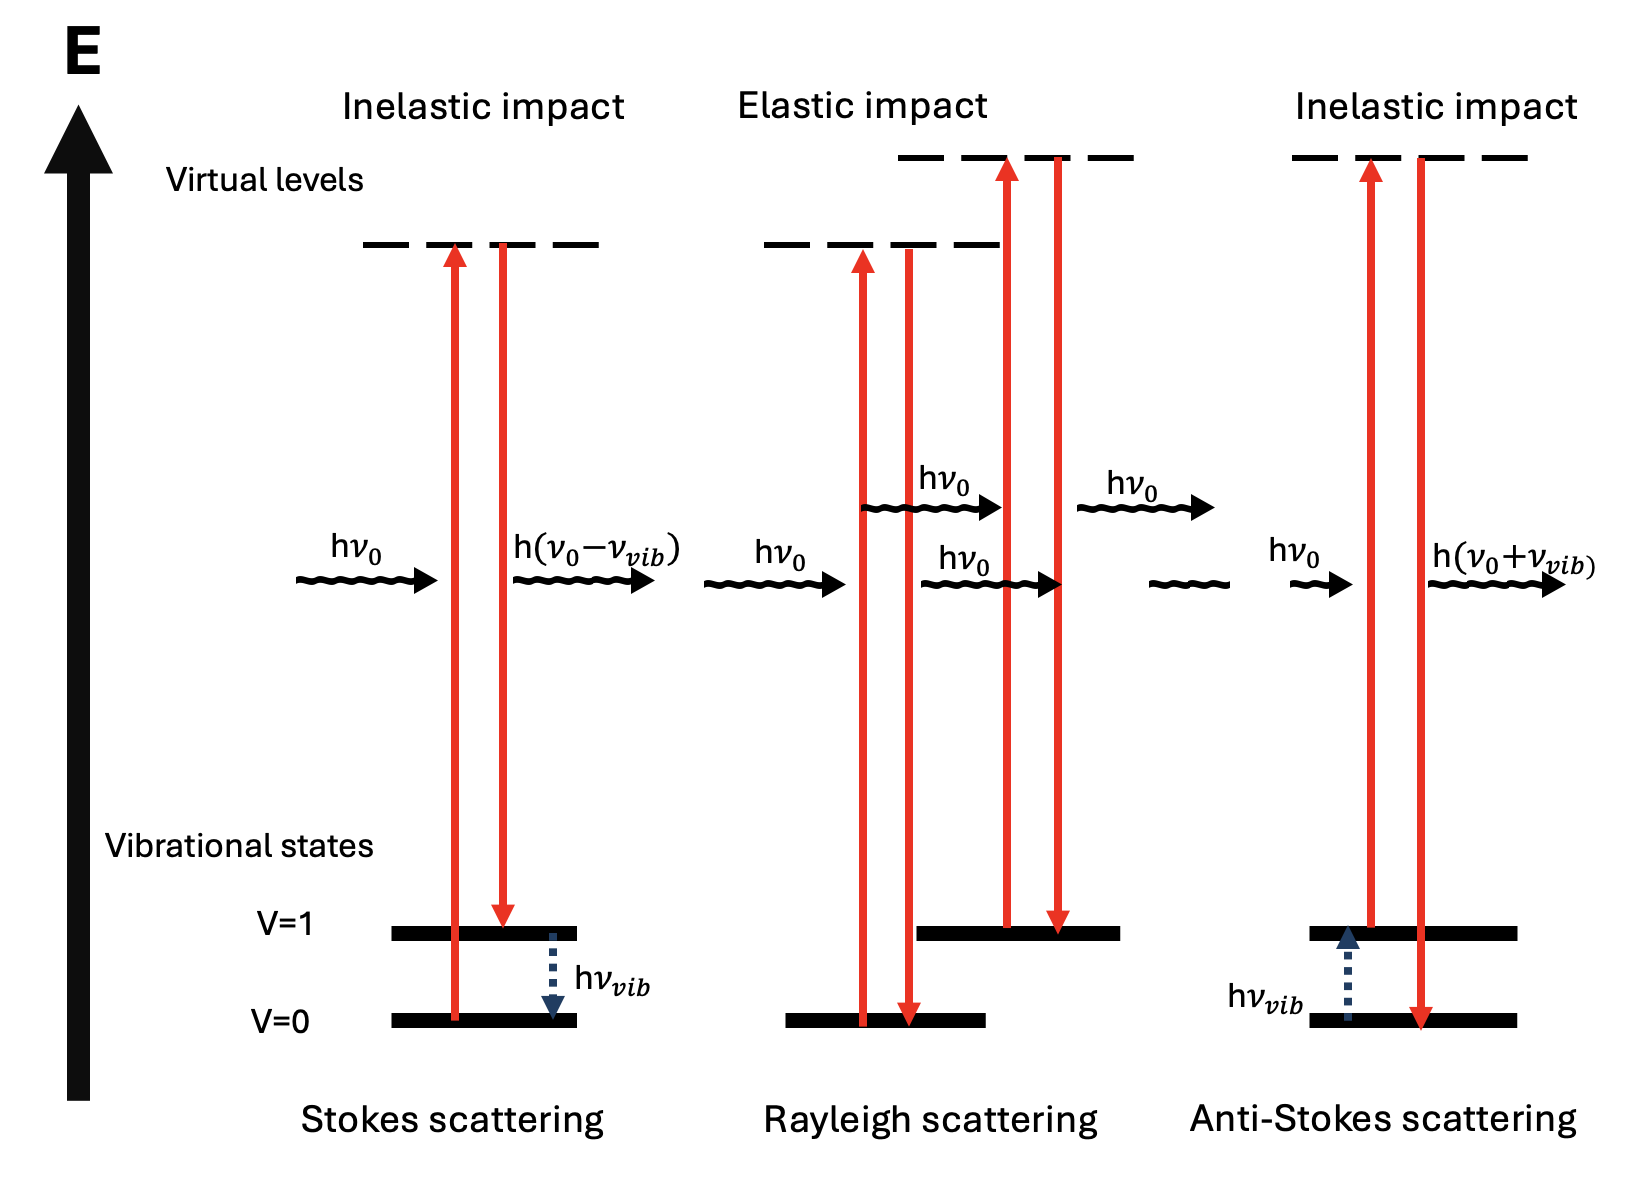
\includegraphics[width=\textwidth]{images/theory/qm_scattering.png}
    \caption{Energy model of the photon molecule collision}
\end{figure}


\newpage

\section{Material and Methods}\label{mat_met}
\subsection{Setup Requirements}

\begin{figure}[ht]
    \centering
    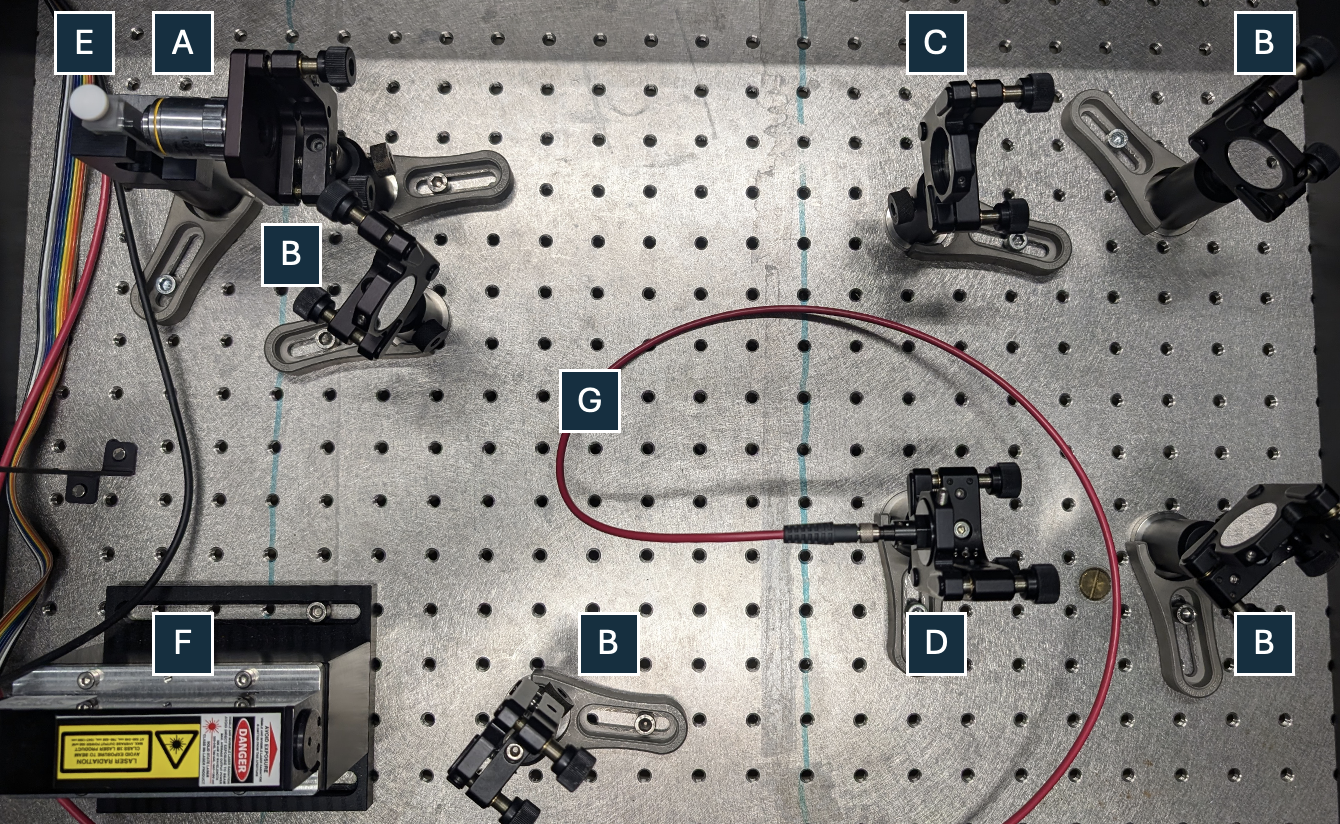
\includegraphics[width=\textwidth]{images/setup_graphics/setup_photo_numbered.png}
    \caption{Graphic of the setup used. A) Objective; B) Mirror; C) Notch filter; D) Optical fibre coupler; E) Sample; F) Laser; G) Optical Cable}
    \label{fig:setup_photo_numbered}
\end{figure}


\subsection{Setup}

\begin{figure}[ht]
    \centering
    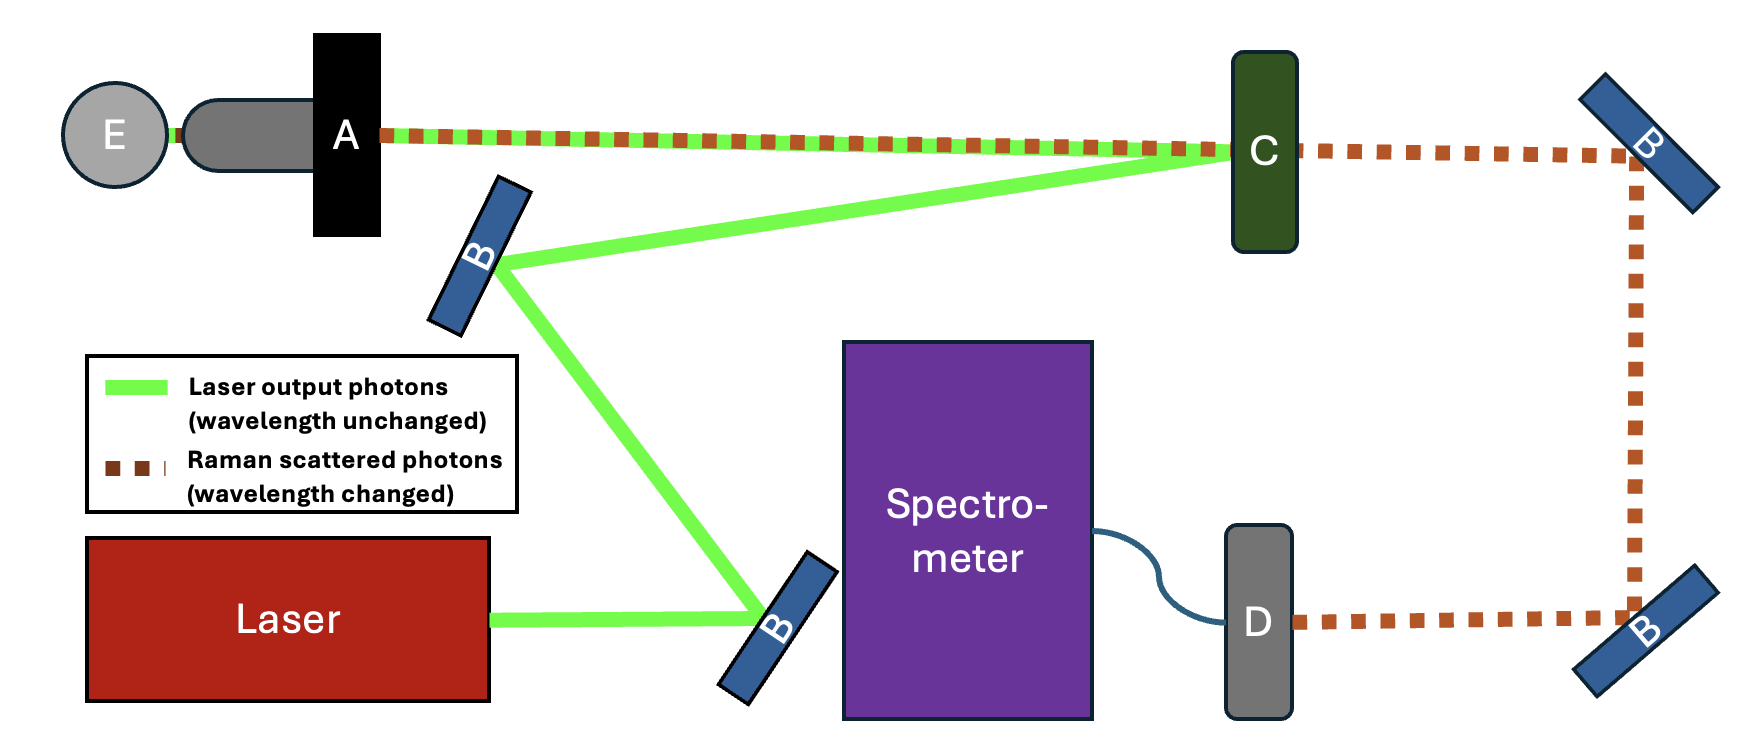
\includegraphics[width=\textwidth]{images/setup_graphics/setup_graphic.png}
    \caption{Graphic of a setup with the optical path. A) Objective; B) Mirror; C) Notch filter; D) Optical fibre coupler; E) Sample}
    \label{fig:setup_graphic}
\end{figure}

A setup for Raman spectroscopy (see Figure \ref{fig:setup_graphic}) uses a laser as the source of excitation radiation, since it has to be monochromatic in order for the raman scattered photons to be visible. By using several mirrors (B), the light is directed to a notch filter (C), which reflects almost all of the photons with a certain wavelength, which is notch-specific. The notch filter has to be selected so that it reflects the original (laser) wavelength. The reflected photons are directed towards a sample (E). Since only a small amount of photons get Raman scattered, it is essential to try to gather them efficiently, so an objective (A) is used to capture the photons, but also to focus the laser light onto the sample surface. The reflected and scattered light that passes back through the objective hits the notch filter again, where the Raman scattered photons pass through while the others get reflected. After passing through the notch filter, mirrors reflect the photons onto an optical fibre coupler, which collects them into an optic fibre to bring them to a spectrometer where they will get recorded as a spectrum.

\newpage

\subsubsection{Laser}
The acronym laser, which stands for "Light Amplification by Stimulated Emission of Radiation" was coined in 1959 by Gordon Gould.
A laser beam is a stream of photons, all of which have the same wavelength and phase. 

\bigskip

In quantum mechanics, electrons in atoms have certain discrete energy levels they can occupy. The higher the energy level, the more energy the atom has. Spontaneously, the atom can transition to a lower energy level, which is when the energy difference between the two levels is released in form of electromagnetic radiation, so a photon. This is called spontaneous emission. In contrast, stimulated emission when a passing photon interacts with the excited electron and causes it to transition to a lower energy level, which creates a photon. The passing photon has to have the same energy as the newly created one, and the created photon also has the same phase as the other. This creates a chain reaction, more and more photons are created if there are enough atoms in an excited state.\cite{wikilaser} \cite{wikistimlaser}

\bigskip

\begin{figure}[ht]
    \centering
    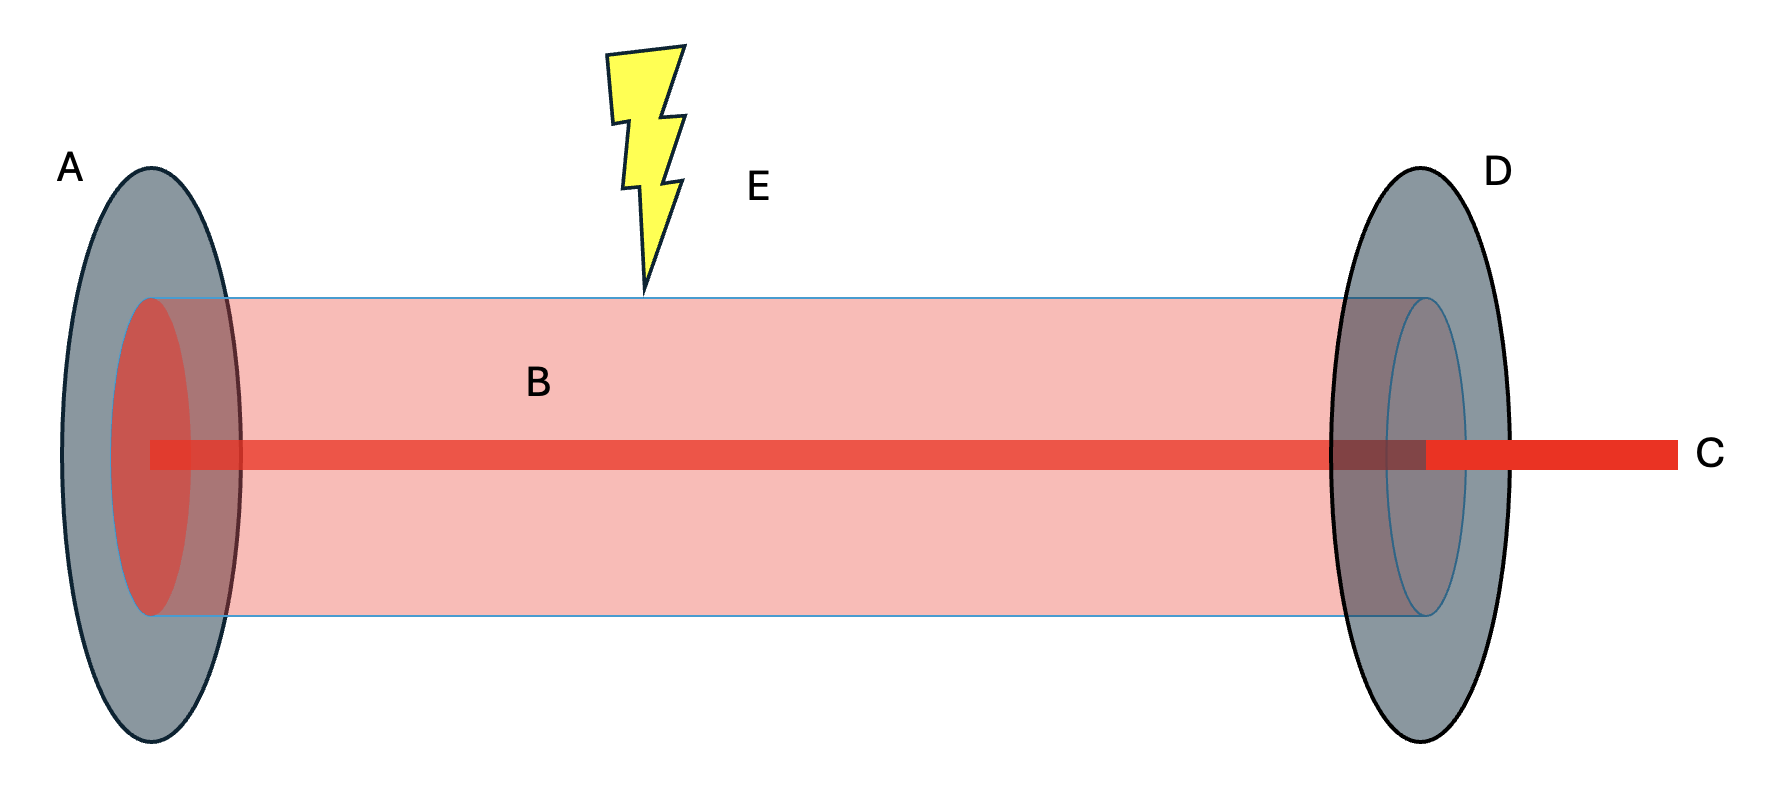
\includegraphics[width=\textwidth]{images/setup_graphics/laser.png}
    \caption{Graphic of a simplified laser: A) full mirror; B) gain medium; C) laser beam; D) partial mirror; E) laser pumping energy;}
    \label{fig:laser}
\end{figure}


In a typical laser (see Figure \ref{fig:laser}), energy (E) is pumped into a so called gain medium (B), usually either by an outside light source or electric field. This process is either continuous or pulsed. When the amount of atoms in one excited state exeeds that of atoms in some lower state, more photons are released than absorbed, the light is amplified. This state is called population inversion. The gain medium is placed between a full mirror (A), which reflects the photons, and a partial mirror (D), which lets some photons through. These photons make up the laser beam (C).\cite{wikilaser} \cite{wikistimlaser}

\newpage

\subsubsection{Notch Filter}
HELP

\newpage
\subsubsection{Optical Spectrometer}


\begin{figure}[ht]
    \centering
    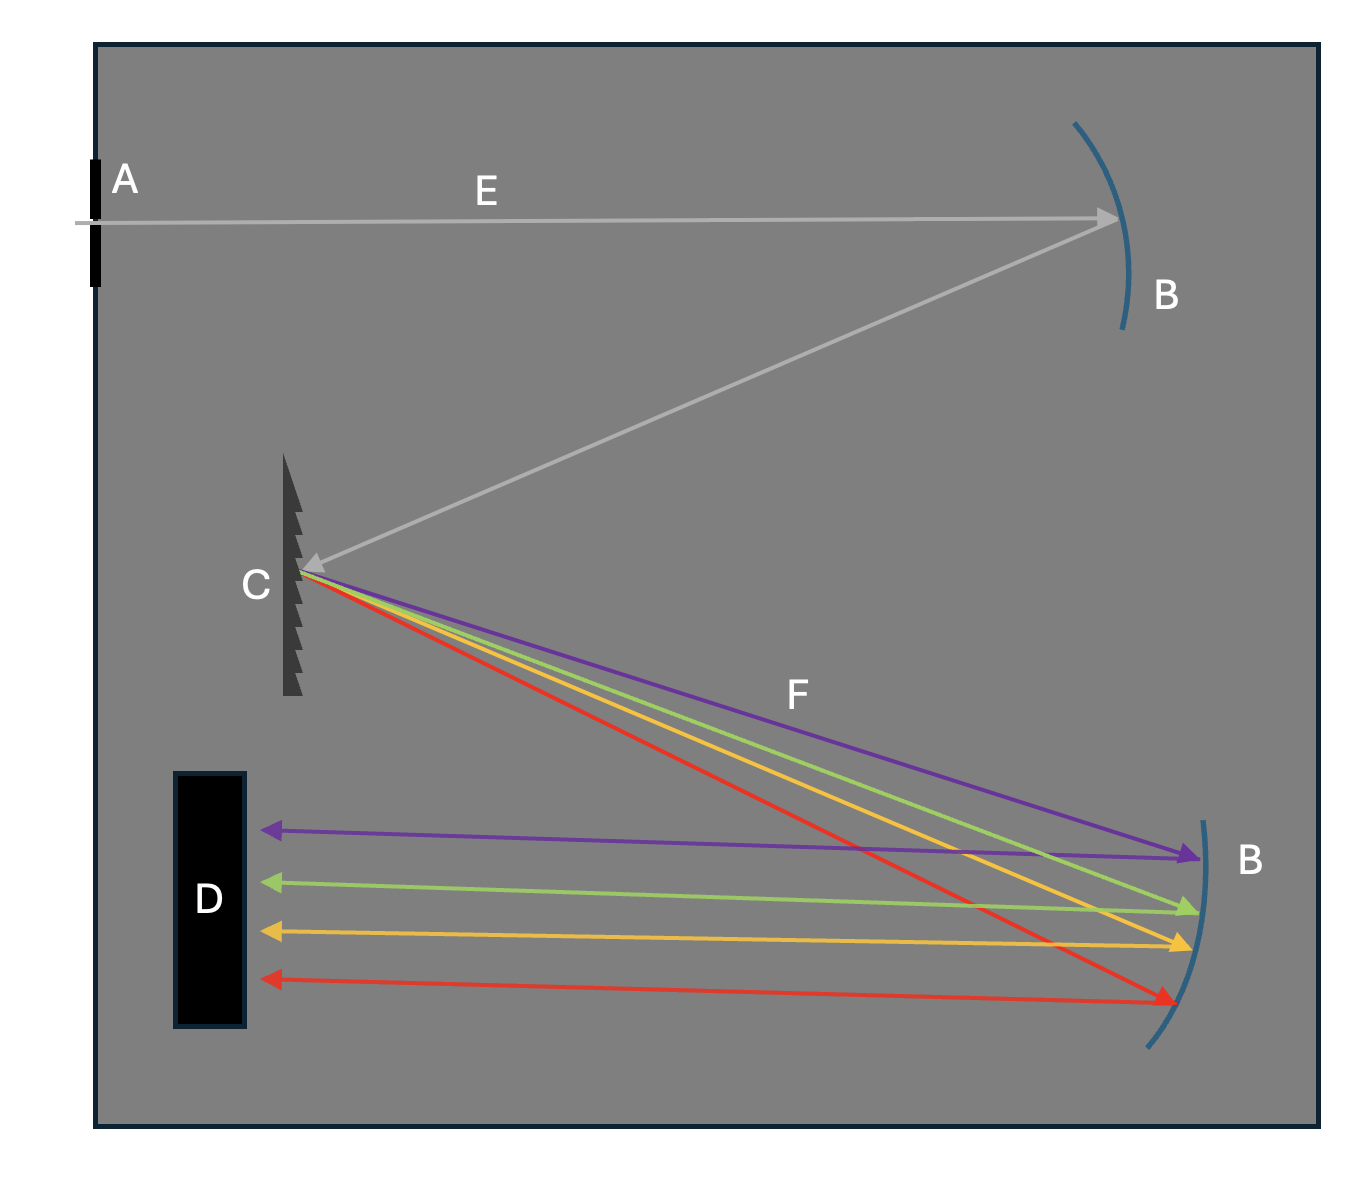
\includegraphics[width=0.9\textwidth]{images/setup_graphics/spectrometer.png}
    \caption{Graphic of a spectrometer A) Entrance slit; B) Mirrors; C) Optical grating; D) CCD detector; E) Incident light; F) Diffracted light}
    \label{fig:spectrometer}
\end{figure}

There exist different types of spectrometers, used to measure light intensity, charges, electron energies and other parameters of samples. Raman spectroscopy uses an opticl spectometer. An optical spectrometer is a device that is used to record and measure light intensity as a version its wavelength. This means that it separates light by wavelength over a fixed period of time. Some spectrometers can also measure the polarization of incident light, which can be used in certain types of Raman spectroscopy, it is specifically essential when Raman spectroscopy is used of crystals. \cite{RSAA} \cite{wikioptspec}

\bigskip

A typical spectrometer (see Figure \ref{fig:spectrometer}) functions in the following way: Light (E) enters the spectrometer through a small entrance slit (A). There it is reflected onto an optical grating (C), which will be discussed in the next chapter. This optical grating separates the light by wavelenghts (F), which are once again reflected onto a CCD detector (D). It records the incident photons and this paper will not address the way the CCD detector is built and the physics behind it's functions.\cite{wikigrating}

\paragraph{Optical Grating}

\begin{wrapfigure}{l}{0.4\textwidth} %this figure will be at the right
    \centering
    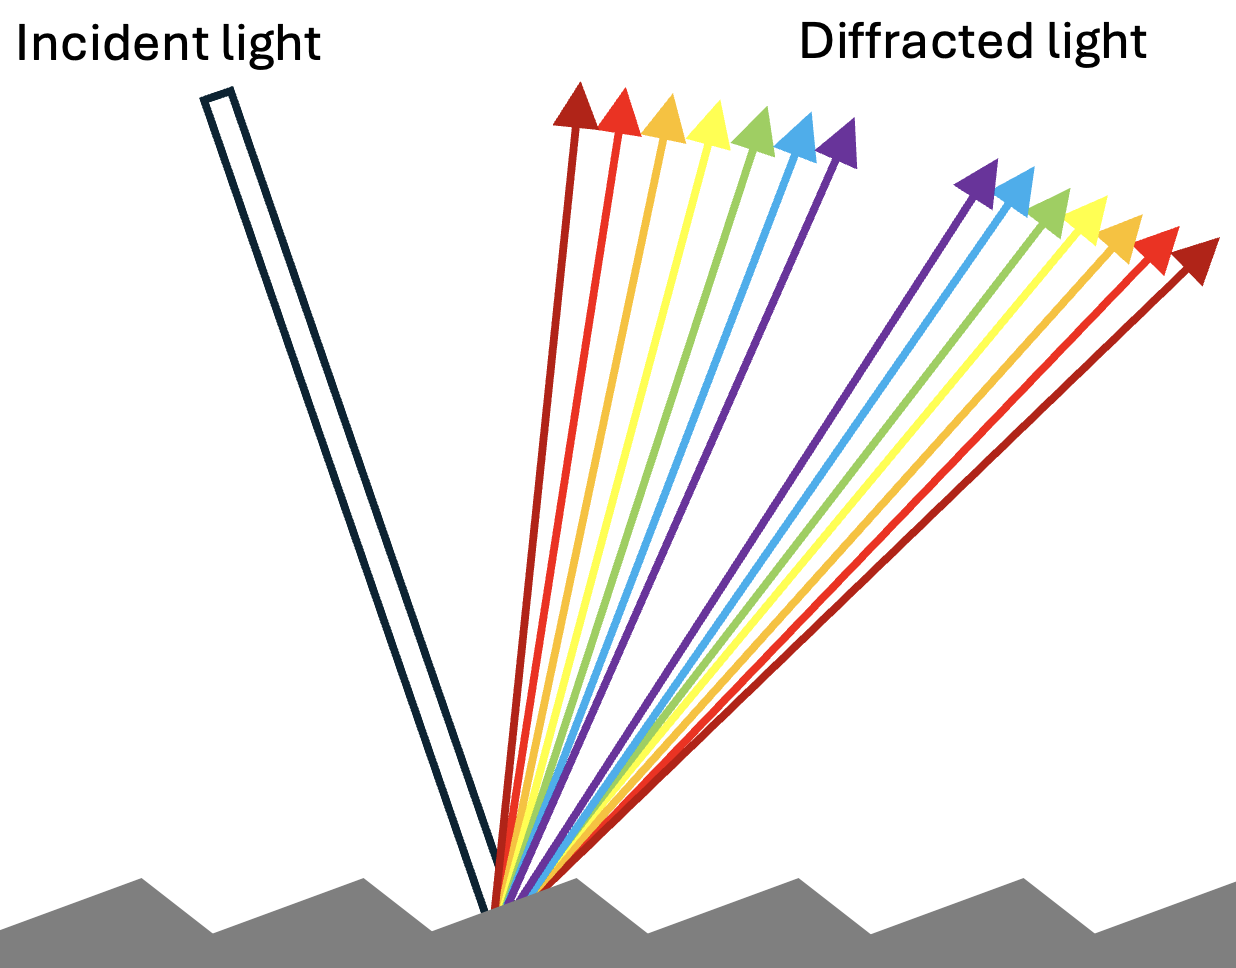
\includegraphics[width=0.3\textwidth]{images/setup_graphics/optical_grating.png}
    \caption{Graphic of an optical grating, simplified}
    \label{fig:grating}
    \vspace{-20pt}
\end{wrapfigure}

An optical grating is used to separate white light by wavelength. Generally, gratings can be separated into two types: reflection and transmission gratings. A reflection grating diffracts light back into the plane of incidence, while a transmission grating transmits it. 
\begin{wrapfigure}{r}{0.5\textwidth}
    \centering
    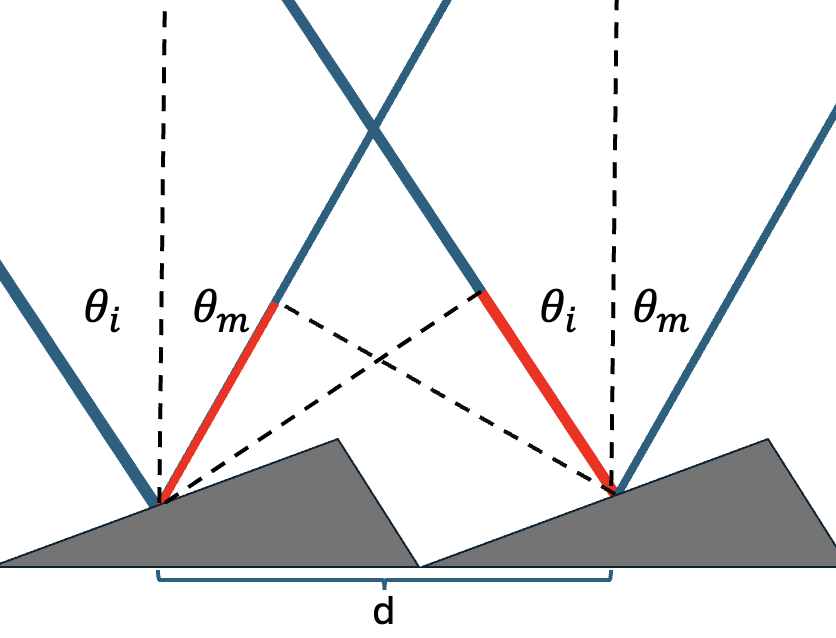
\includegraphics[width=0.4\textwidth]{images/setup_graphics/grating_graphic.png}
    \caption{Graphic of a reflection grating: d: distance between grooves, \(\theta_i\): incident angle light; \(\theta_m\): angle with constructive interference; Blue: distance in the path of both photons that is the same; Red: differences in path distance}
    \label{fig:grating_graphic}
\end{wrapfigure}
Figure \ref{fig:grating} depicts a reflection grating. Spectrometers usually use reflection gratings, they will be discussed.

\bigskip

A reflection based diffraction grating is a plate with grooves which are tightly spaced. The shape of the grooves can differ, Figure \ref{fig:grating} shows a triangular grooving, but mor wave-like groovings are also common. Generally, the distance between the grooves is not given but can be calculated from the usually given groove density value. Typical gratings have a groove density value between 30 and 5000 grooves per mm.

\bigskip


When photons hit a diffraction grating, they are diffracted into all directions. Since a photon is an electromagnetic wave with wavelength \(\lambda\), they interfere with each other. The interference can be constructive or destructive, depending on whether the waves are in phase or out of phase. In order to be constructive, the diffenrence in path of two photons of the same wavelength has to be a multiple of the wavelength. The angles at which the interference is constructive can be calculated with the wavelength, incident angle and groove spacing.


\begin{equation}
     sin(\theta_m)-sin(\theta_i)=\frac{m \lambda}{d}
 \end{equation}

\(\theta_i\): Incident angle (see Figure \ref{fig:grating_graphic})\\
\(\theta_m\): Diffraction angle (see Figure \ref{fig:grating_graphic})\\
m: Order of diffraction\\
\(\lambda\): Wavelength incident light\\
D: Distance beetween grooves (see Figure \ref{fig:grating_graphic})

\newpage

\subsection{Additional Material}

In addition, to properly align the mirrors, a second, much weaker laser was used. It was inserted in place of the optical fibre coupler and used to align the mirrors between the notch filter and the optical coupler. 

\bigskip

The intensity of the Raman shifted light which is reflected by those mirrors is too weak to be observed and used to align the mirrors, which is the reason the second laser was used. Its wavelength differs from the main laser so that it can pass through the notch filter which is chosen based on the wavelength of the main laser
\bigskip

While working with the laser, laser safety glasses were worn. 

\subsubsection{Laptop with OceanView 1.6.7}

\begin{wrapfigure}{r}{0.4\textwidth}
    \vspace{-20pt}
    \centering
    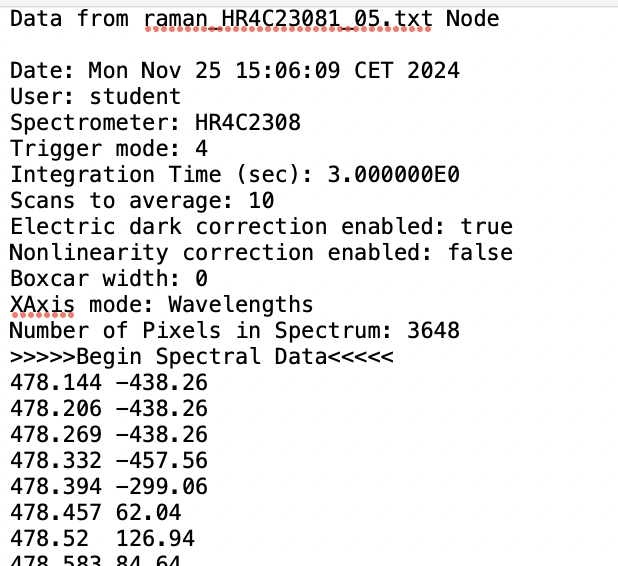
\includegraphics[width=0.4\textwidth]{images/data_raman.png}
    \vspace{-30pt}
    \caption{Beginning of the exported Raman data file}
    \label{fig:raman_txt}
    \vspace{-10pt}
\end{wrapfigure}
The spectrometer was connected to a laptop with the software OceanView 1.6.7, which was used to record spectra of the samples. The data points were exported as a text file, see Figure \ref{fig:raman_txt}. The file contains information to the data, when it was recorded, what integration time was used and how many scans were averaged out, among other parameters. The spectral data is then evaluated and plotted using python code, see Figure \ref{fig:python} in the Appendix.

\bigskip


\newpage


\subsection{Practical setup}
\subsection{Fine-tuning and Intensity Optimisation}

\newpage

\section{Results and Discussion}
The raw data would show the intensity of light, measured as the absolute amount of photons, as a function of the wavelength. This makes the spectrum dependent on the initial wavelength of the laser light. A Raman spectrum is not dependent on the initial wavelength and shows the intensity as a function of the difference in wavenumber of the observed photons to the initial laser light, the Raman shift. In order to be able to compare the experimental results to literature, certain calculations have to be performed.

\subsection{Evaluation of the Measured Data}

    As mentioned in Section \ref{mat_met}, the data is exported as a text file with pairs of numbers. The first number refers to the wavelength at which an intensity was recorded, the second number specifies that intensity. The specific wavelengths reported stay the same for all measurements, since they are predefined by the spectrometer.


    \begin{equation}
        \widetilde{\nu} = \frac{1}{\lambda}
    \end{equation}

    \(\widetilde{\nu}\): Wavenumber\\
    \(\lambda\): Wavelength\\

  The wavenumber \(\widetilde{\nu}\) is the inverse of th wavelength, and in order to calculate the raman shift the difference between the experimentally recorded wavenumber and the wavenumber of the incident laser radiation has to be calculated.

    \begin{equation} \label{eq:1}
        \widetilde{\nu}_r = \frac{1}{\lambda_i} - \frac{1}{\lambda_r}
    \end{equation}

    \(\widetilde{\nu}_r\): Raman shift\\
    \(\lambda_i\): Wavelength laser light, initial wavelength\\
    \(\lambda_r\): Wavelength raman scattered photons

    \bigskip

    In order to get more accurate results, a background spectrum was recorder, without a sample but while the laser was active. These values are subtracted from the initial intensities before calculating the wavenumbers. 

    \begin{equation} \label{eq:2}
        I_{res}=I_r-I_b
    \end{equation}

    \( I_{res}\): Resulting intensity\\
    \(I_r\): Intensity Raman scattered photons\\
    \(I_b\): Intensity background measurement

    \bigskip

    The intensities that are calculated with the Equation \ref{eq:2} are then plotted as a function of the Raman shift calculated in Equation \ref{eq:1}. This task was done using a program written in python, see Figure \ref{fig:python} in the Appendix.

\subsection{Errors}
The width of a raman peak can be a result of different things, one of the possibilities is that two close peaks overlap, which results in their convolution, and are indistinguishable from each other and only identifiable as one broad, potentially asymmetric peak. This can result in errors when measuring the wavelength with the maximum intensity value and comparing it to literature. A spectrometers ability to resolute close-lying peaks is a very important parameter. Spectrometers are not perfect and produce an apparent spectral broadening of the purely monochromatic wavelength Half Width at Half Maximum (HWHM), half the distance between the two points on the curve with half of the maximal value, can be used to measure resolution.

\bigskip

Different literature sources provide different peak values for the same molecules, not all literature sources mention all peaks that appear so differences appear, but generally they are relatively small. 

\newpage


\subsection{Comparison to Literature}

\paragraph{Dichloromethane}

\begin{wrapfigure}{r}{0.4\textwidth} %this figure will be at the right
    \centering
    \vspace{-20pt}
    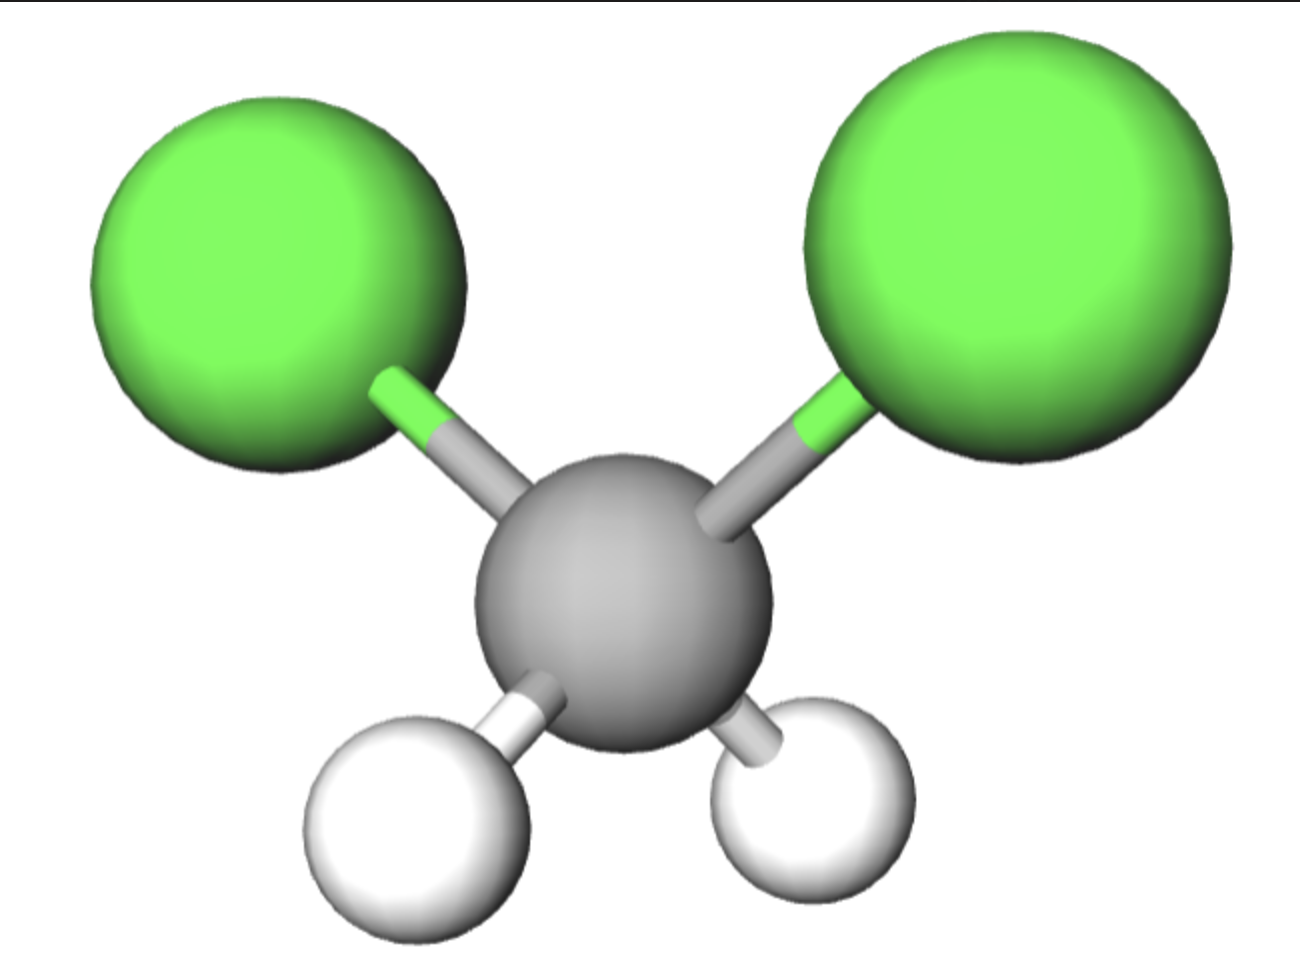
\includegraphics[width=0.3\textwidth]{images/raman_spectra/dcm_i.png}
    \caption{Dichloromethane, ball and stick model. Green: chlorine; gray: carbon; white: hydrogen}
    \label{fig:dcm_i}
\end{wrapfigure}


    Figures \ref{fig:dcm_x} and \ref{fig:dcm_l} show experimental and literature spectra of dichloromethane, CH\(_2\)Cl\(_2\), which is one carbon atom with two covalent bonds to hydrogen atoms and two to chloride atoms, see Figure \ref{fig:dcm_i}. This 5-atomic molecule has 3\(\cdot\)5-6, so 9 vibrational modes, all of which are raman active. Table \ref{table:dcm} compares the recorded peaks to literature values, as well as notes the assigned vibrational modes. 

    \begin{table}[h]
    \begin{center}
        \vspace{10pt}
        \begin{tabular}{|c|c|c|}
         \hline
         Exp. Wavelength (\( cm^{-1} \) ) & Lit. Wavelength  (\( cm^{-1} \) ) & Assingment  \\ 
         \hline
         175 & - & - \\
         295 & 282 & CCl\(_2\) bending \\ 
         714 & 713 & CCl symmetric stretching\\
         750 & 748 & CCl asymmetric stretching\\
         - & 893 & CH\(_2\) rocking \\
         1167 & 1153 & CH\(_2\) twisting\\
         - & 1255 & CH\(_2\) wagging\\
         1434 & 1467 & CH\(_2\)  scissoring\\
         2999 & 2996 & CH symmetric stretching \\
         3067 & 3019 & CH asymmetric stretcing \\
         \hline
        \end{tabular}
        \caption{Comparison of experimental and literature \cite{dcml} values, as well as assingment of peaks in a Raman spectrum of dichloromethane by wavenumber. The experimental value represents the maximum of the measured peak }
        \label{table:dcm}
        \vspace{-15pt}
    \end{center}
    \end{table}

    Table \ref{table:dcm} shows that the measured values match the literature values. The missing peaks at 893 and 1255 \( cm^{-1}\) could be explained by the fact that they might just be too weak to be mentioned, as the corresponding regions in Figure \ref{fig:dcm_x} show slight elevations. The different peaks in Figure \ref{fig:dcm_x} are more pronounced, which might be the result of better quality equipment, specifically the spectrometer, which is able to differenciate between peaks that are very close together. The peaks without assignment might stem from rotational frequencies and not vibrational frequencies.


    \bigskip

    The small peaks with a negative raman shift were not mentioned in the table, but they are the results of Anti-Stokes scattering.

    \bigskip

    The literature values used in Table \ref{table:dcm} and the Figure \ref{fig:dcm_l} are not the same, so there are some differences, but they are small. Figre \ref{fig:dcm_l} is used to demonstrate the relative intensities of the raman bands.

    \newpage
     
    \begin{figure}[h]
        \centering
        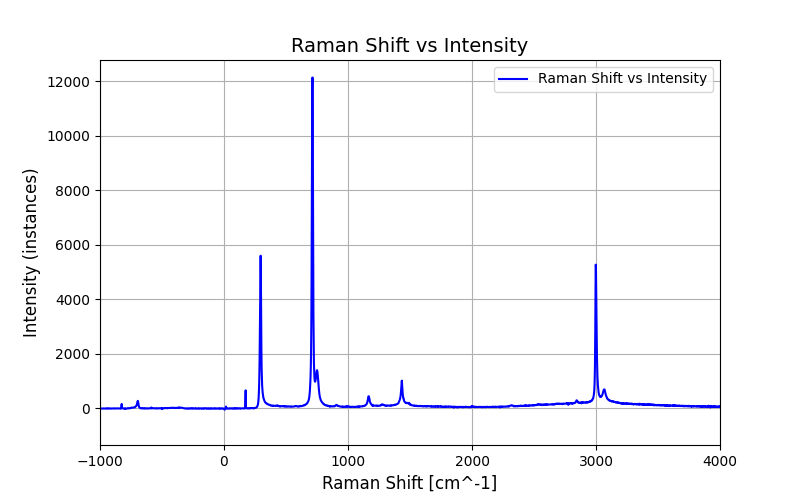
\includegraphics[width=\textwidth]{images/raman_spectra/raman_shift_DCM.png}
        \caption{Experimental Raman spectrum of dichloromethane}
        \label{fig:dcm_x}
    \end{figure}

    \begin{figure}[h]
        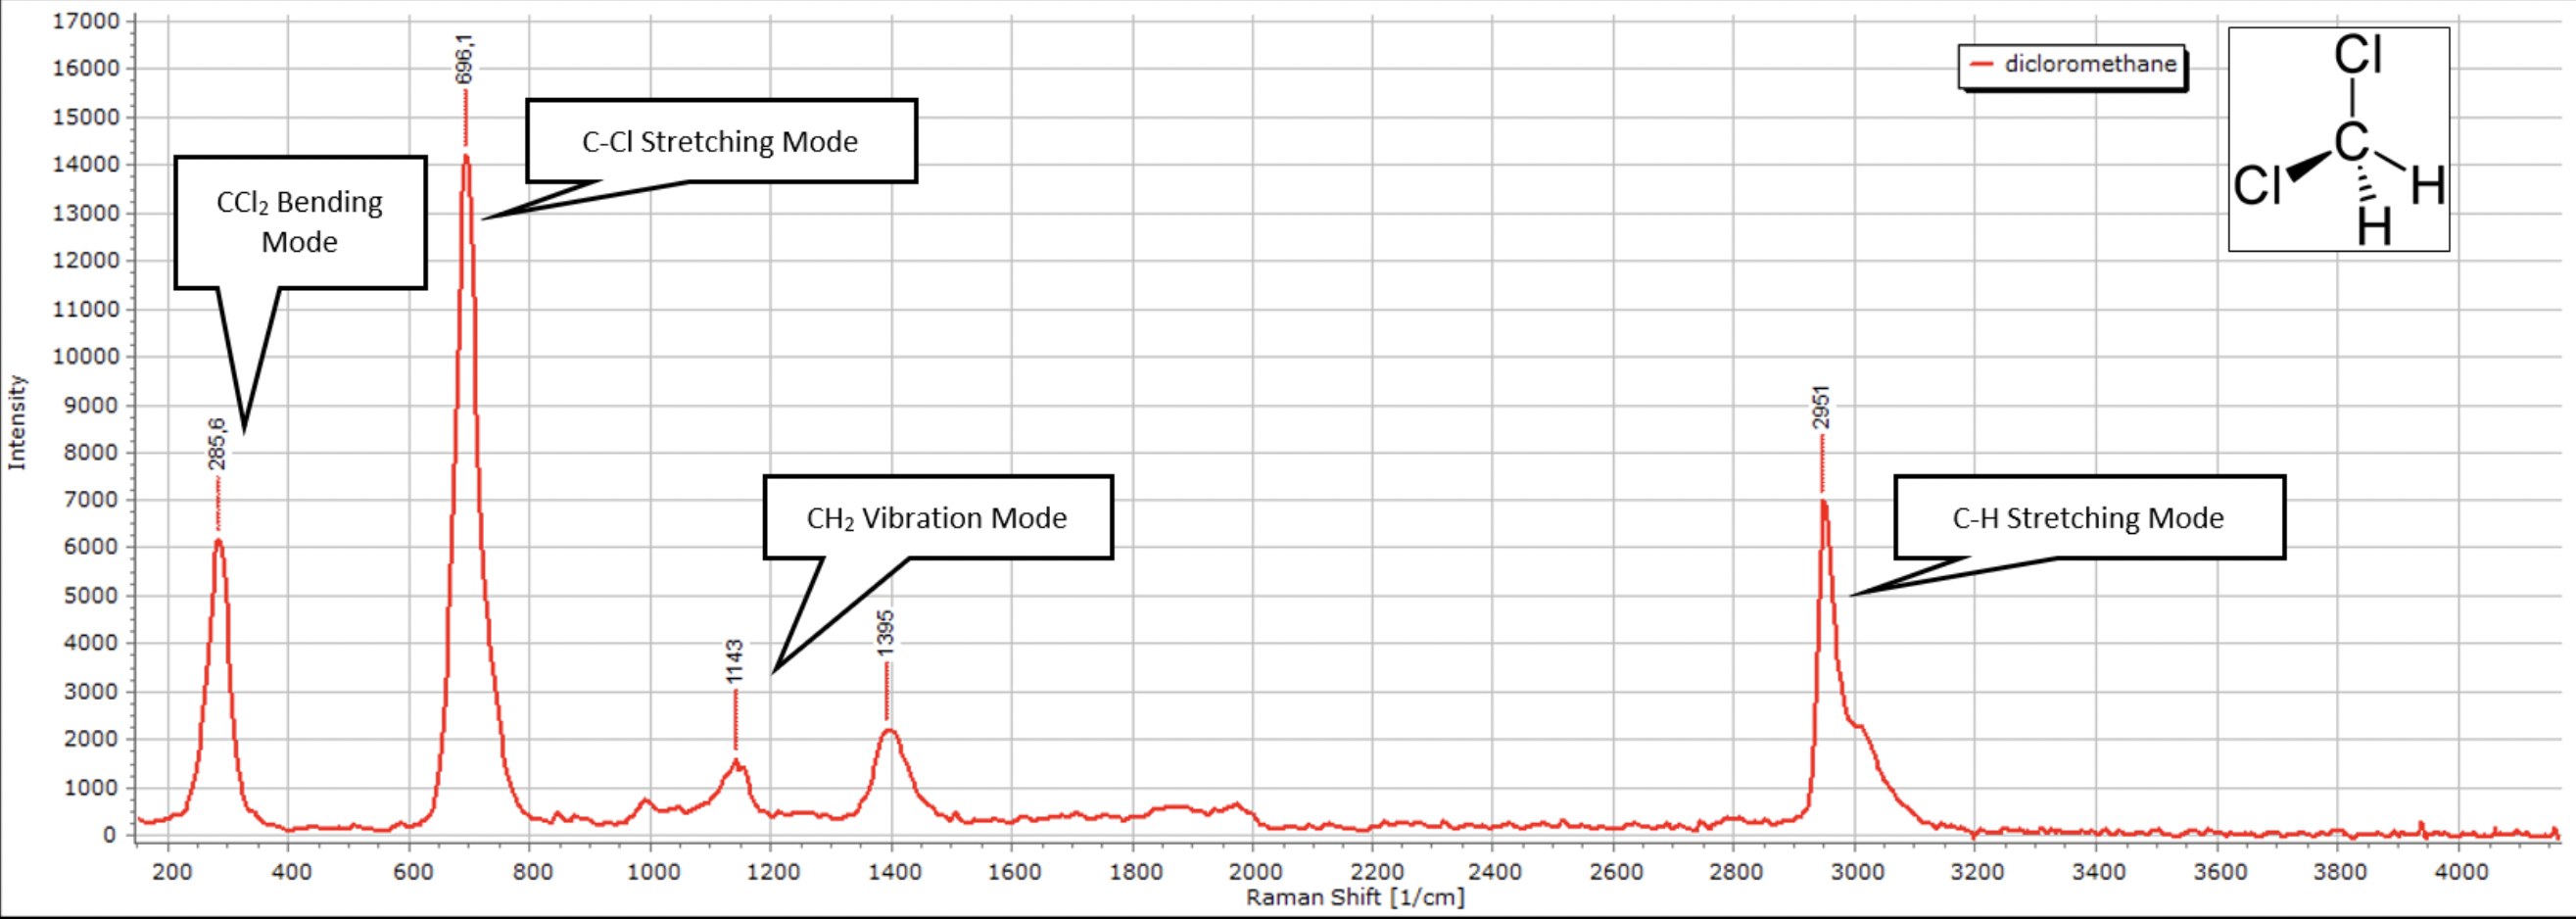
\includegraphics[width=\textwidth]{images/lit_raman/dichloromethane.png}
        \caption{Literature Raman spectrum of dichloromethane \cite{spectrumdcm}}
        \label{fig:dcm_l}
    \end{figure}

    \newpage

\paragraph{Ethanol}

    \begin{wrapfigure}{radiation}{0.5\textwidth} %this figure will be at the right
        \centering
        \vspace{-20pt}
        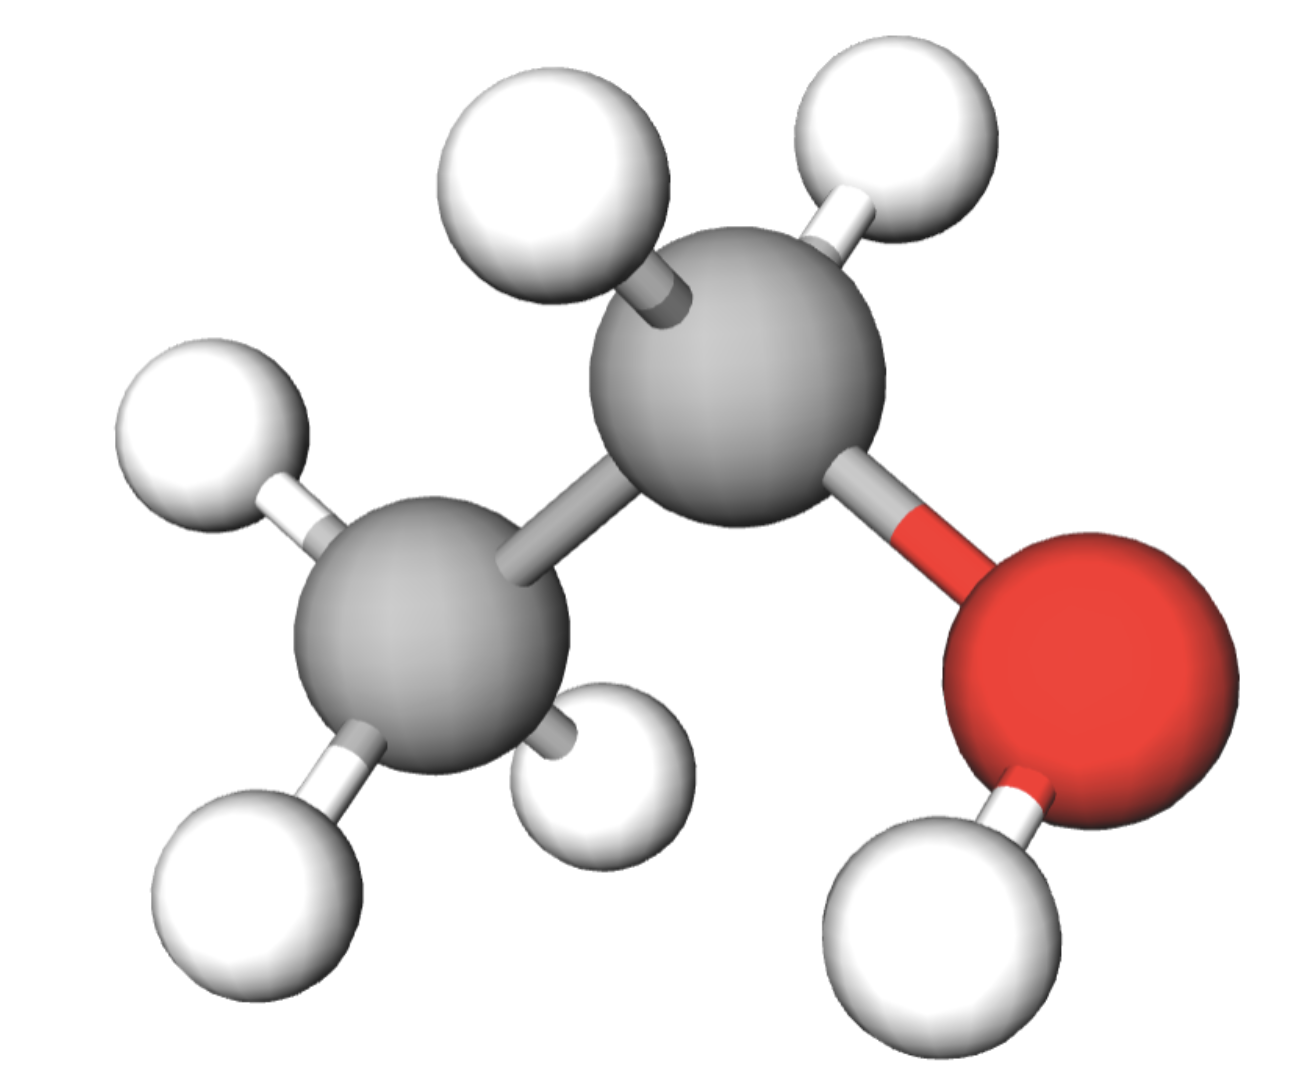
\includegraphics[width=0.4\textwidth]{images/raman_spectra/eth_i.png}
        \caption{Ethanol, ball and stick model. Red: oxygen; gray: carbon; white: hydrogen}
        \label{fig:eth_i}
    \end{wrapfigure}


    Figures \ref{fig:eth_x} and \ref{fig:eth_l} show experimental and literature spectra of ethanol, C\(_2\)H\(_6\)O, see Figure \ref{fig:eth_i}.  Table \ref{table:eth} compares the recorded peaks to literature values, as well as notes the assigned vibrational modes. Raman spectrography can be used to differenciate ethanol from methanol, which is important because while normal alcohol contains ethanol, methanol is toxic to humans.

    \begin{table}[h]
    \begin{center}
        \vspace{15pt}
        \begin{tabular}{|c|c|c|}
         \hline
         Exp. Wavelength (\( cm^{-1} \) ) & Lit. Wavelength  (\( cm^{-1} \) ) & Assingment  \\ 
         \hline
         442 & - & - \\
         894 & 883 & CC stretchung \\ 
         1064 & 1050 & CO stretching\\
         1107 & 1093 & CO stretching\\
         1287 & 1277 & - \\
         1465 & 1454 & CH\(_3\) bending\\
         2891& 2885 &  CH stretching mode\\
         2942 & 2929 & CH stretching mode\\
         2985 & 2974 & CH stretching mode\\
         
         \hline
        \end{tabular}
        \caption{Comparison of experimental and literature \cite{ethl1} \cite{ethl2} values, as well as assingment of peaks in a Raman spectrum of ethanol by wavenumber. The experimental value represents the maximum of the measured peak }
        \label{table:eth}
    \end{center}
    \end{table}

    Table \ref{table:eth} shows that the measured values match the literature values. Sadly, not all bands were assigned and the bands 2891, 2942 and 2985 cm\(^{-1}\) were not differenciated between. Same as with dichloromethane, the peaks are more differenciated in Figure \ref{fig:eth_x} than in the literature Figure \ref{fig:eth_l}. The OH stretching mode was not as clearly identifyable and wasn't recorded for that reason.

    \bigskip
    
    The raman spectrum for methanol wouldn't have the very visible peak at around 900 cm\(^{-1}\) which comes from a CC stretching mode.

    The literature values used in Table \ref{table:eth} and the Figure \ref{fig:eth_l} are not the same, so there are some differences, but they are small. Different sources record slightly different values. 

    

    \newpage

    \begin{figure}[h]
        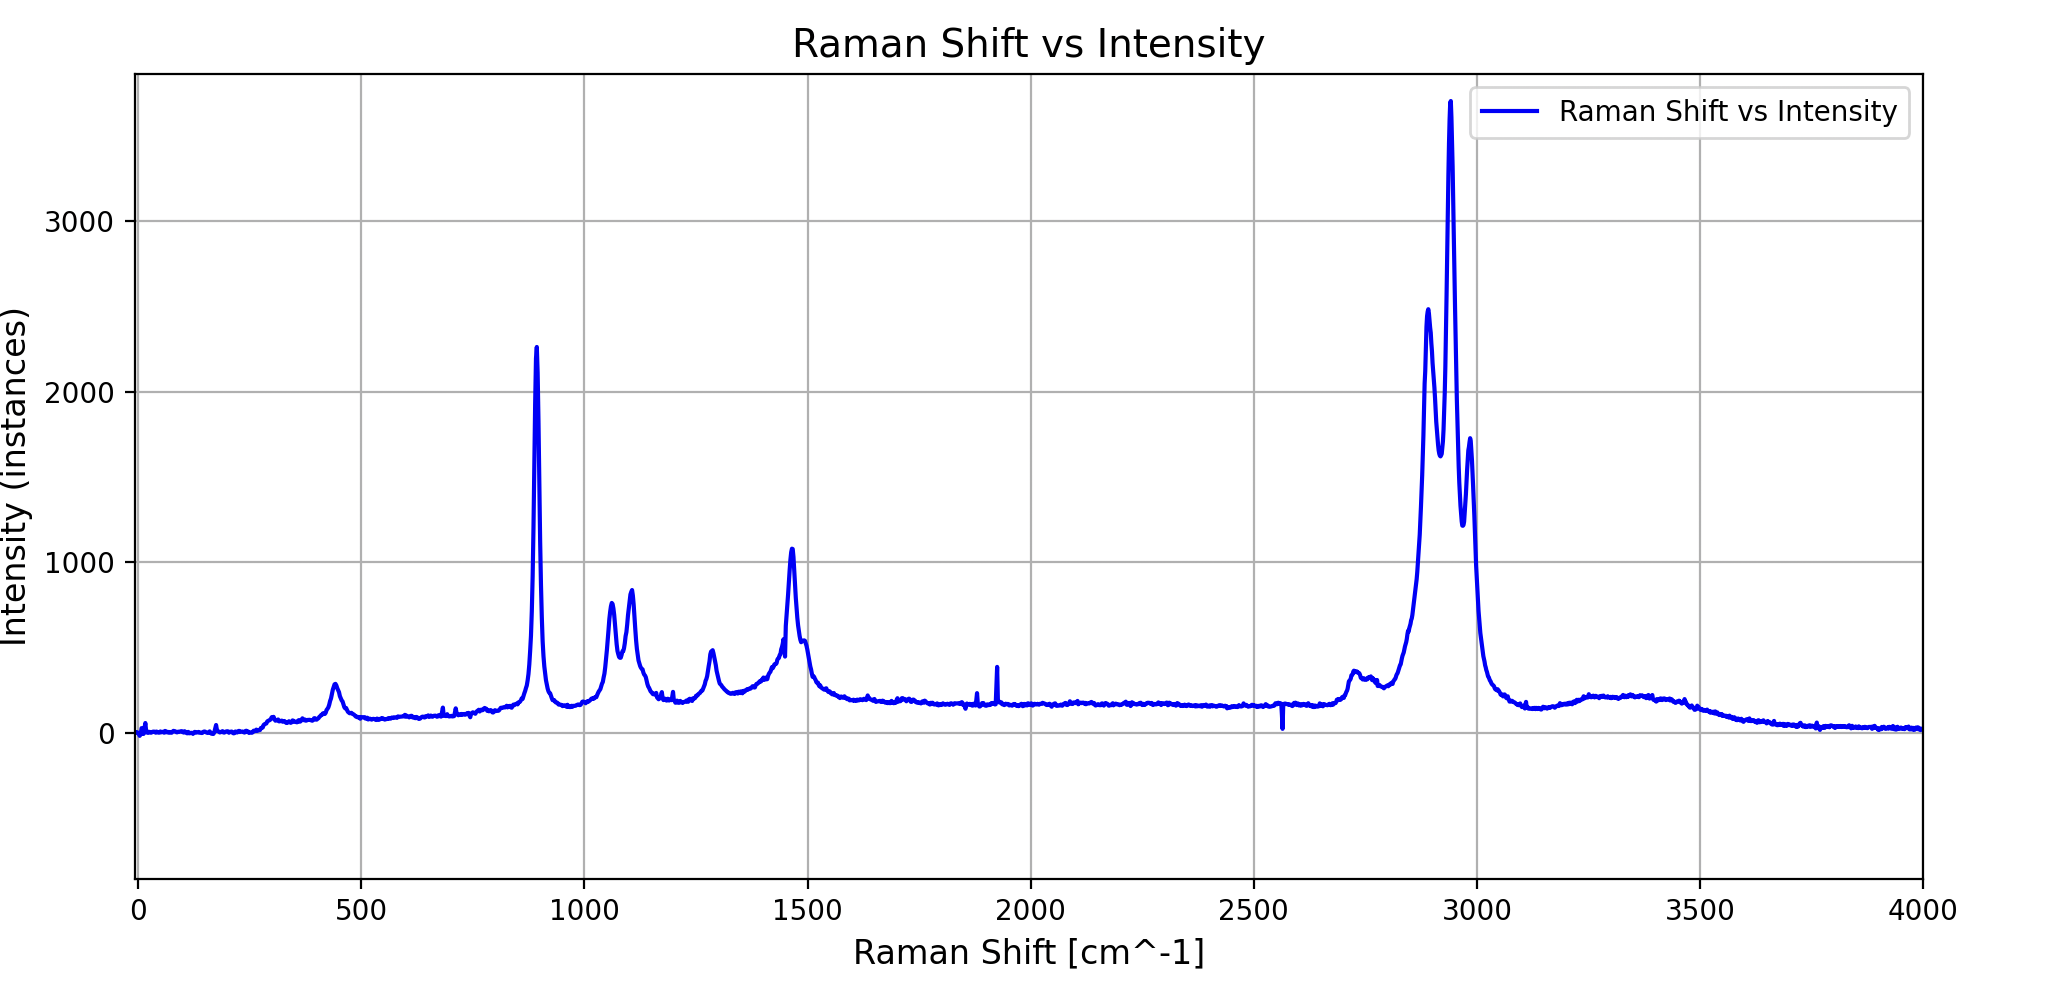
\includegraphics[width=\textwidth]{images/raman_spectra/raman_shift_ethanol.png}
        \caption{Experimental Raman spectrum of ethanol}
        \label{fig:eth_x}
        \vspace{10pt}
    \end{figure}


    \begin{figure}[h]
        \centering
        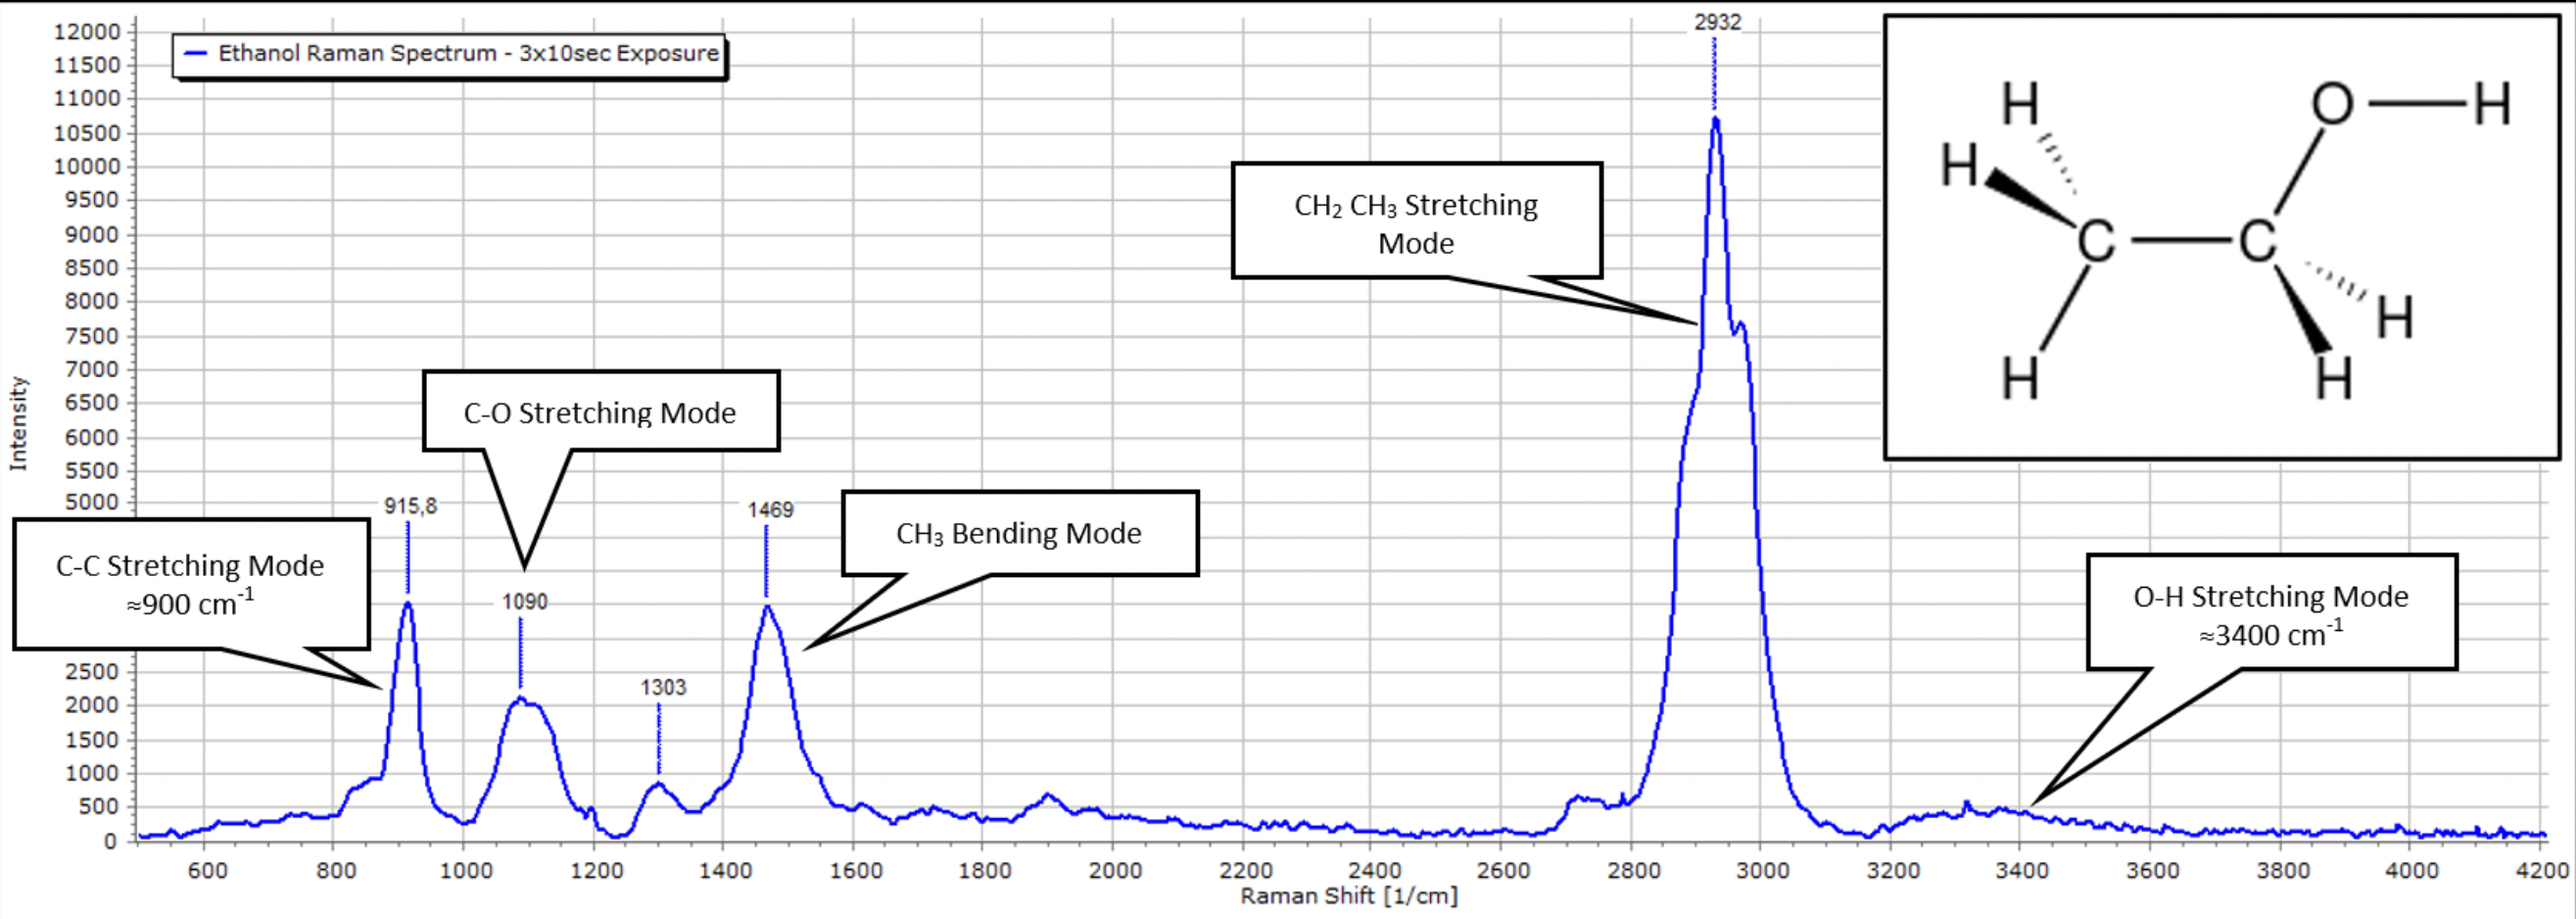
\includegraphics[width=\textwidth]{images/lit_raman/ethanol.png}
        \caption{Literature Raman spectrum of ethanol \cite{spectrumet} }
        \label{fig:eth_l}
    \end{figure}

    \newpage

    \paragraph{Polyethylene (PE)}

    \begin{wrapfigure}{radiation}{0.5\textwidth} %this figure will be at the right
        \centering
        \vspace{-20pt}
        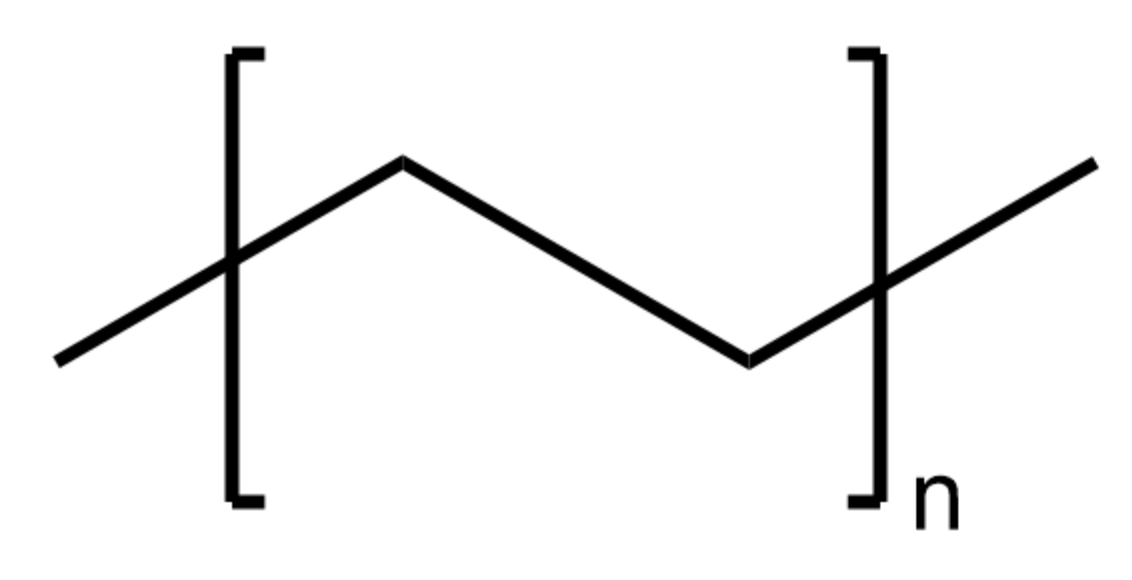
\includegraphics[width=0.4\textwidth]{images/raman_spectra/pe_i.png}
        \caption{Polyethylene, skeleton model}
        \label{fig:pe_i}
    \end{wrapfigure}


    Figures \ref{fig:pe_x} and \ref{fig:pe_l} show experimental and literature spectra of polyethylene, (C\(_2\)H\(_2\))\(_n\), see Figure \ref{fig:pe_i}. \\
    The same unit, C\(_2\)H\(_2\), is repeated an undefined amount of times, which results in a long carbon chain Table \ref{table:eth} compares the recorded peaks to literature values, as well as notes the assigned vibrational modes. 

    \begin{table}[h]
    \begin{center}
        \vspace{15pt}
        \begin{tabular}{|c|c|c|}
         \hline
         Exp. Wavelength (\( cm^{-1} \) ) & Lit. Wavelength  (\( cm^{-1} \) ) & Assingment  \\ 
         \hline
         0 & - & reflections laser light \\
         175 & - & - \\
         1072 & 1062 & CC stretching crystalline\\ 
         1091 & 1079 & CC stretching amorphous\\
         1139 & 1128 & CC stretching\\
         1180 & 1169 & CH\(_2\) rocking\\
         1305 & 1294 & CH\(_2\) twisting\\
         1379 & 1369 & CH\(_3\) wagging amorphous\\
         1428 & 1416 & CH\(_2\) bending \\
         1451 & 1439 & CH\(_2\) bending\\
         1468 & 1462 & CH\(_2\) bending\\
         2861& 2848 &  CH\(_2\) symmetric stretching\\
         2892& 2882 &  CH\(_2\) asymmetric stretching\\
         \hline
        \end{tabular}
        \caption{Comparison of experimental and literature \cite{pel1} \cite{pel2} values, as well as assingment of peaks in a Raman spectrum of polyethylene by wavenumber. The experimental value represents the maximum of the measured peak }
        \label{table:pe}
    \end{center}
    \end{table}

    Table \ref{table:pe} shows that the measured values match the literature values. Since PE is semicrystalline, some values, for example at 1379 cm\(^{-1}\) and 1091 cm\(^{-1}\) correspond to vibrational modes in amorphous regions, some in crystalline, and some, like 1468 cm\(^{-1}\), are influenced by both. Peaks that are exclusive to crystalline structures, like the one at 1428 cm\(^{-1}\), can be used to evaluate the degree of crystallinity.

    \bigskip
    
    The literature values used in Table \ref{table:pe} and the Figure \ref{fig:pe_l} are not the same, so there are some differences, but they are small. Different sources record slightly different values. For PE, often only the peaks between 1000 cm\(^{-1}\) and 1600 cm\(^{-1}\) are looked at, which is the reason for the multiple sources in Table \ref{table:pe}.

    

    \newpage

    \begin{figure}[h]
        \centering
        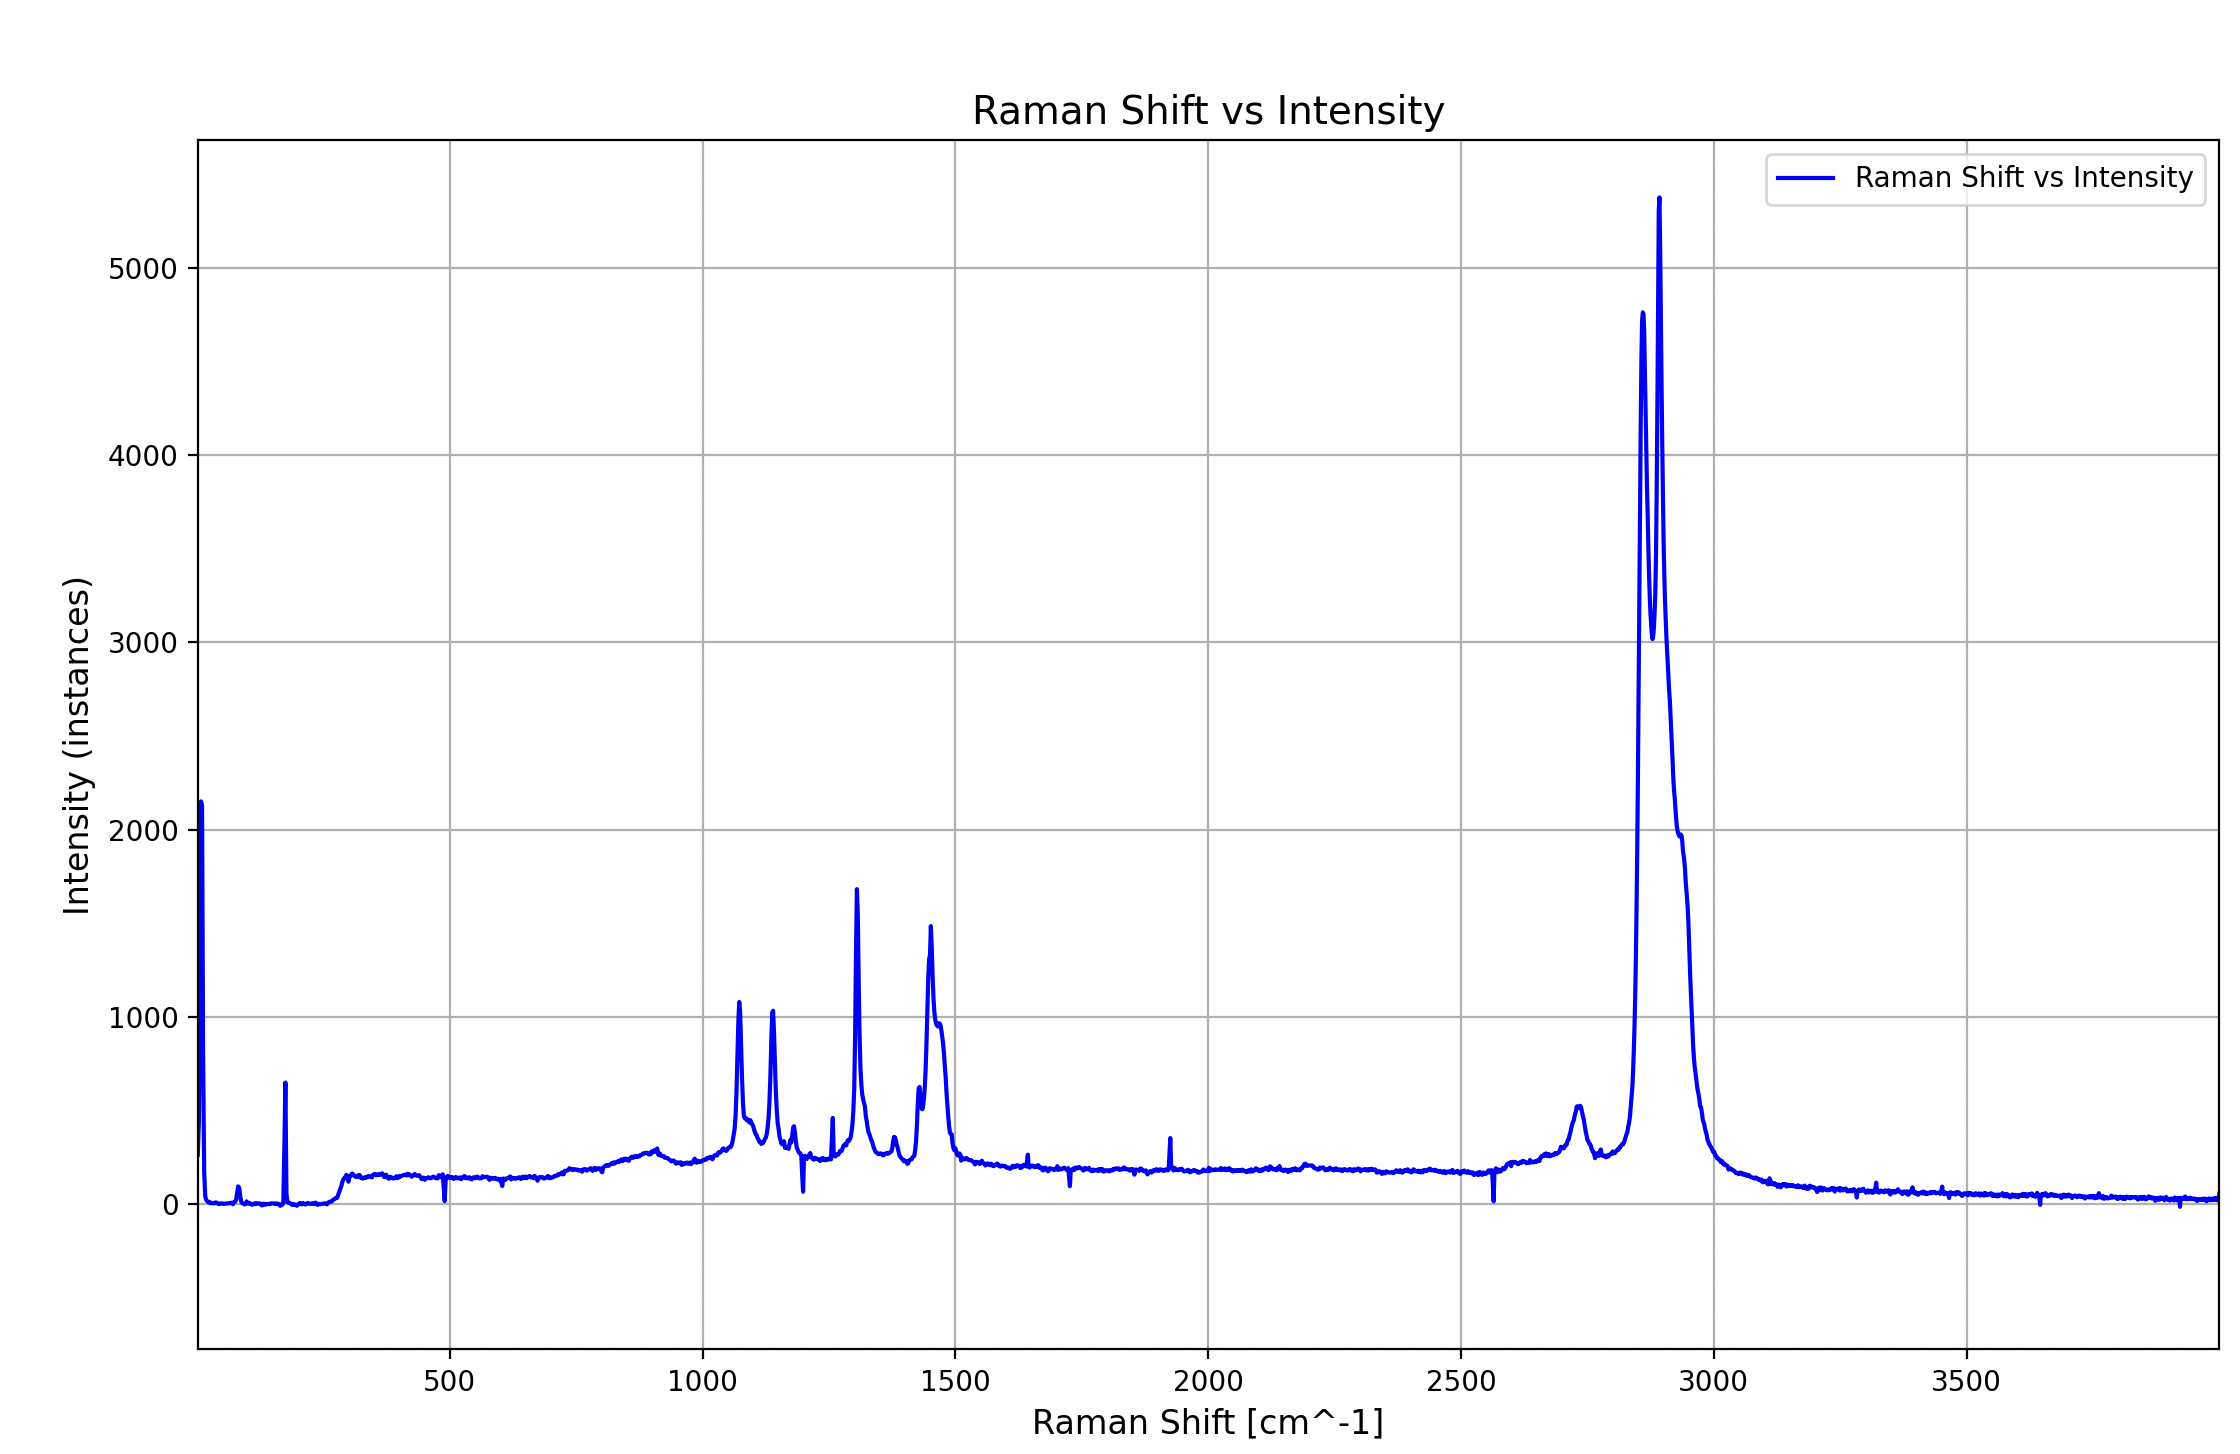
\includegraphics[width=\textwidth]{images/raman_spectra/raman_shift_polyethyleneh.png}
        \caption{Experimental Raman spectrum of polyethylene}
        \label{fig:pe_x}
    \end{figure}

    \begin{figure}[h]
        \centering
        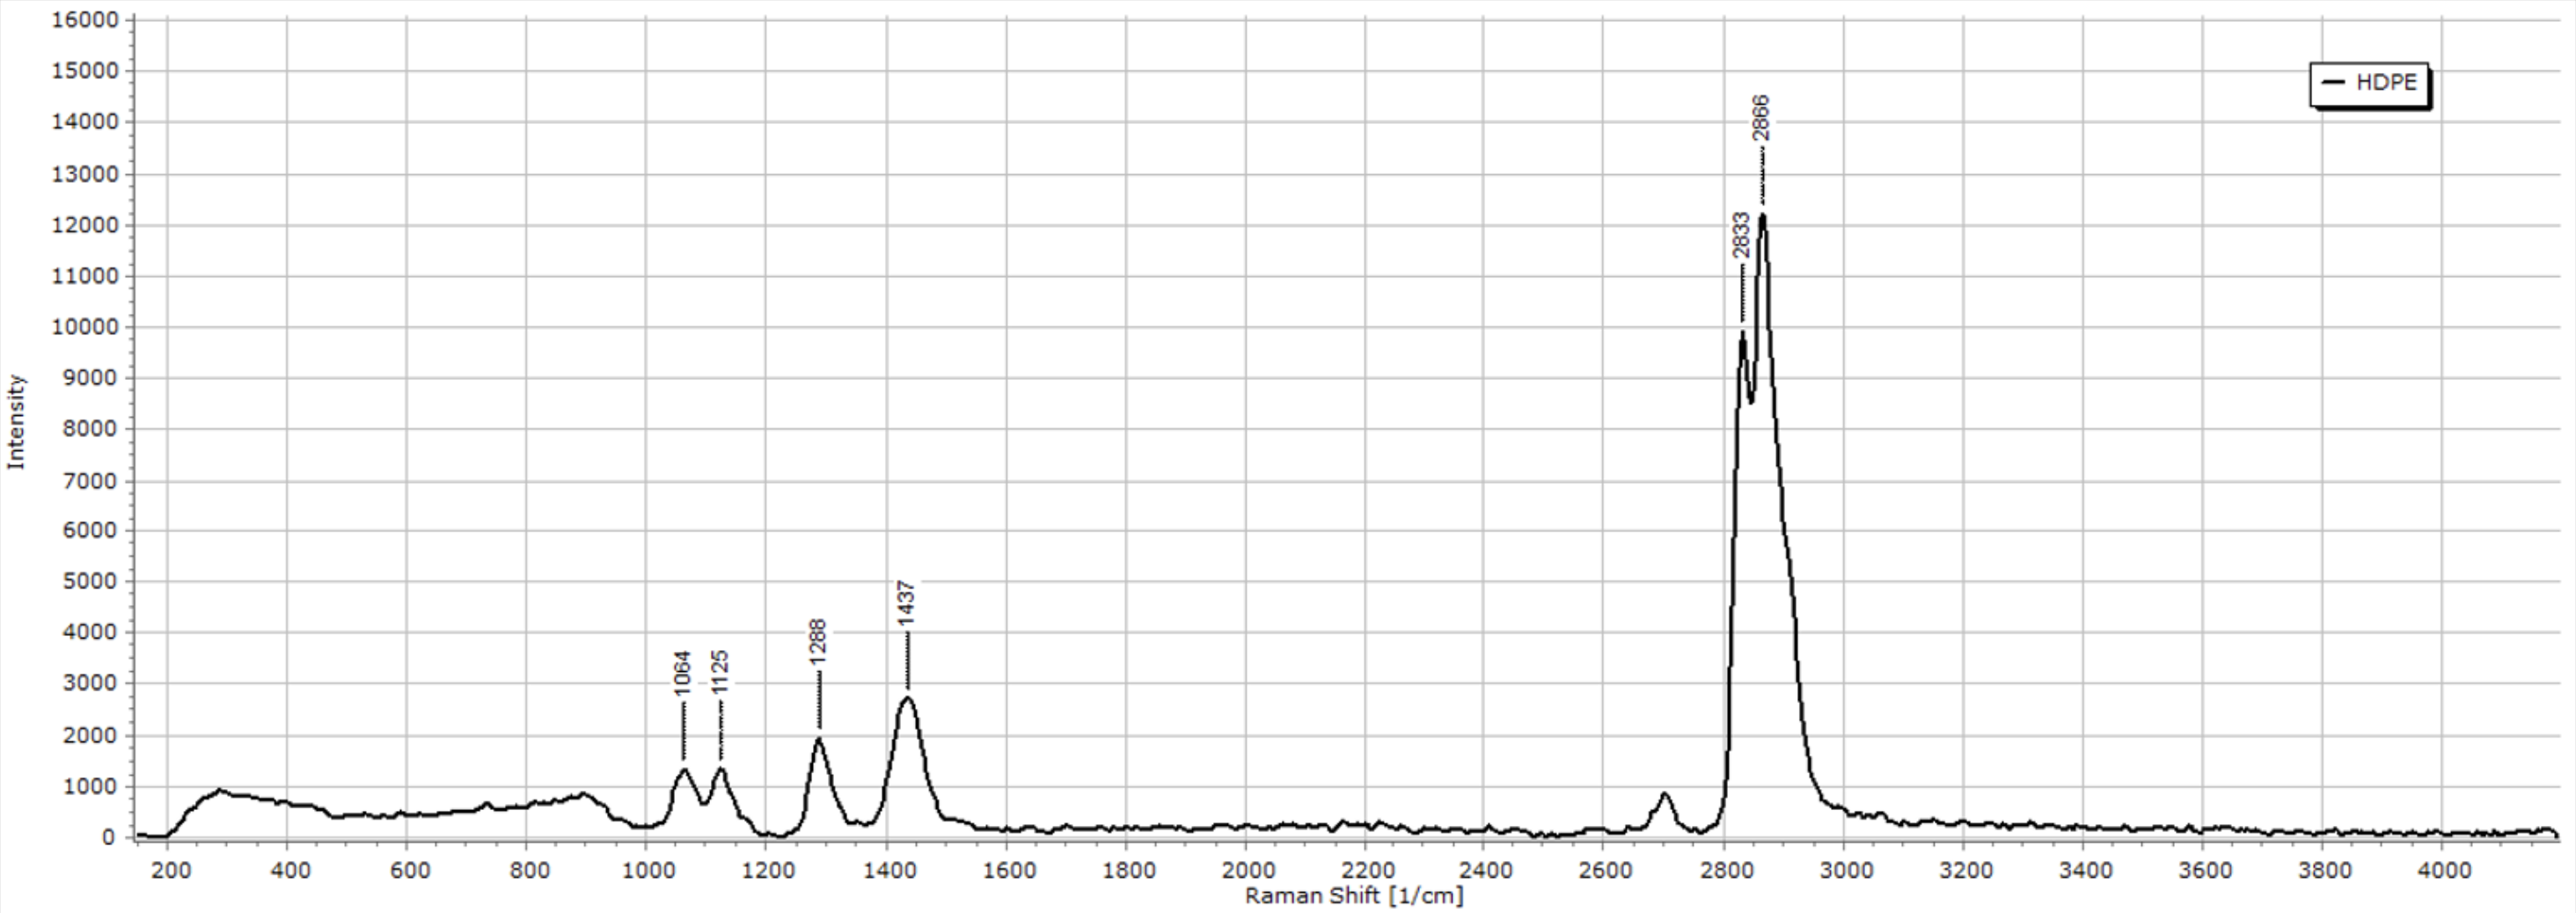
\includegraphics[width=\textwidth]{images/lit_raman/HDPE.png}
        \caption{Literature Raman spectrum of polyethylene \cite{spectrap}}
        \label{fig:pe_l}
    \end{figure}

    \newpage

    \paragraph{Polystyrene (PS)}
    
    \begin{wrapfigure}{radiation}{0.4\textwidth} %this figure will be at the right
        \centering
        \vspace{-20pt}
        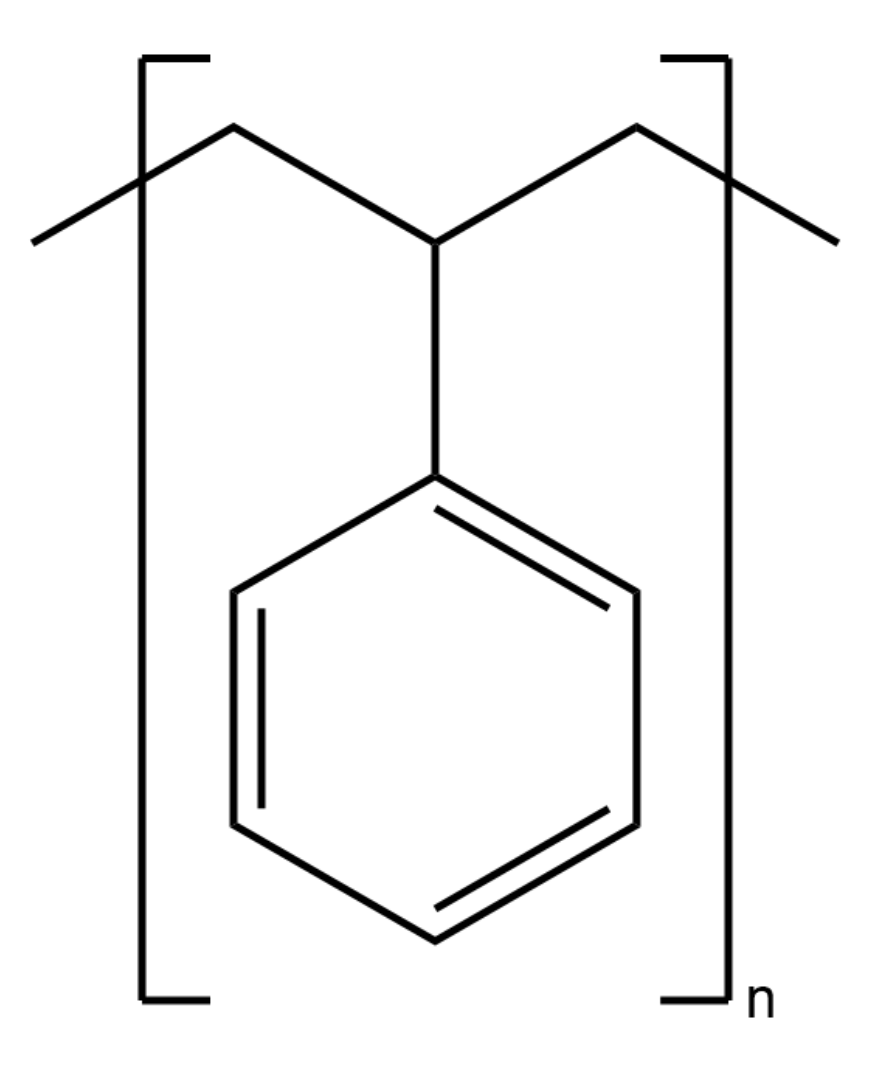
\includegraphics[width=0.3\textwidth]{images/raman_spectra/ps_i.png}
        \caption{Polystyene, skeleton model}
        \label{fig:ps_i}
    \end{wrapfigure}


    Figures \ref{fig:ps_x} and \ref{fig:ps_l} show experimental and literature spectra of polystyrene, (C\(_8\)H\(_8\))\(_n\) see Figure \ref{fig:pe_i}.\\ 
    The unit C\(_8\)H\(_8\), a benzene ring attached to an ethane chain and repeated an undefined number of times, results in a carbon chain with every second carbon atom being attached to a benzene ring. Table \ref{table:eth} compares the recorded peaks to literature values, as well as notes the assigned vibrational modes. 

    \begin{table}[h]
    \begin{center}
        \vspace{15pt}
        \begin{tabular}{|c|c|c|}
         \hline
         Exp. Wavelength (\( cm^{-1} \) ) & Lit. Wavelength  (\( cm^{-1} \) ) & Assingment  \\ 
         \hline
         631 & 621 & ring deformation mode \\
         805 & 795 & CH out-of-plane deformation \\
         1012 & 1001 & ring breathing mode\\ 
         1041 & 1031 & CH in-plane deformation \\
         1165 & 1155 & C-C stretching\\
         1461 & 1450 & H\(_2\) scissoring\\
         1594 & 1583 & C=C stretch\\
         1613 & 1602 & ring-skeletal stretch\\
         2923 & 2915 & CH\(_2\) antisymmetric stretch\\
         3068 & 3060 & CH aromatic stretch  \\
         \hline
        \end{tabular}
        \caption{Comparison of experimental and literature \cite{ps1} \cite{ps2} values, as well as assingment of peaks in a Raman spectrum of polyethylene by wavenumber. The experimental value represents the maximum of the measured peak }
        \label{table:ps}
    \end{center}
    \end{table}

    Table \ref{table:pe} shows that the measured values match the literature values. A greater degree of precision could be achieved by averaging more scans or using longer exposure times, as well as ensuring the absence of any other light during the recording of the spectra.

    \bigskip
    
    The literature values used in Table \ref{table:ps} and the Figure \ref{fig:ps_l} are not the same, so there are some differences, but they are small. Different sources record slightly different values. Often only the peaks up to 2000 cm\(^{-1} \) are considered, which is the reason for the multiple sources in Table \ref{table:ps}. 
    

    \newpage

    \begin{figure}[h]
        \centering
        \makebox[\textwidth][c]{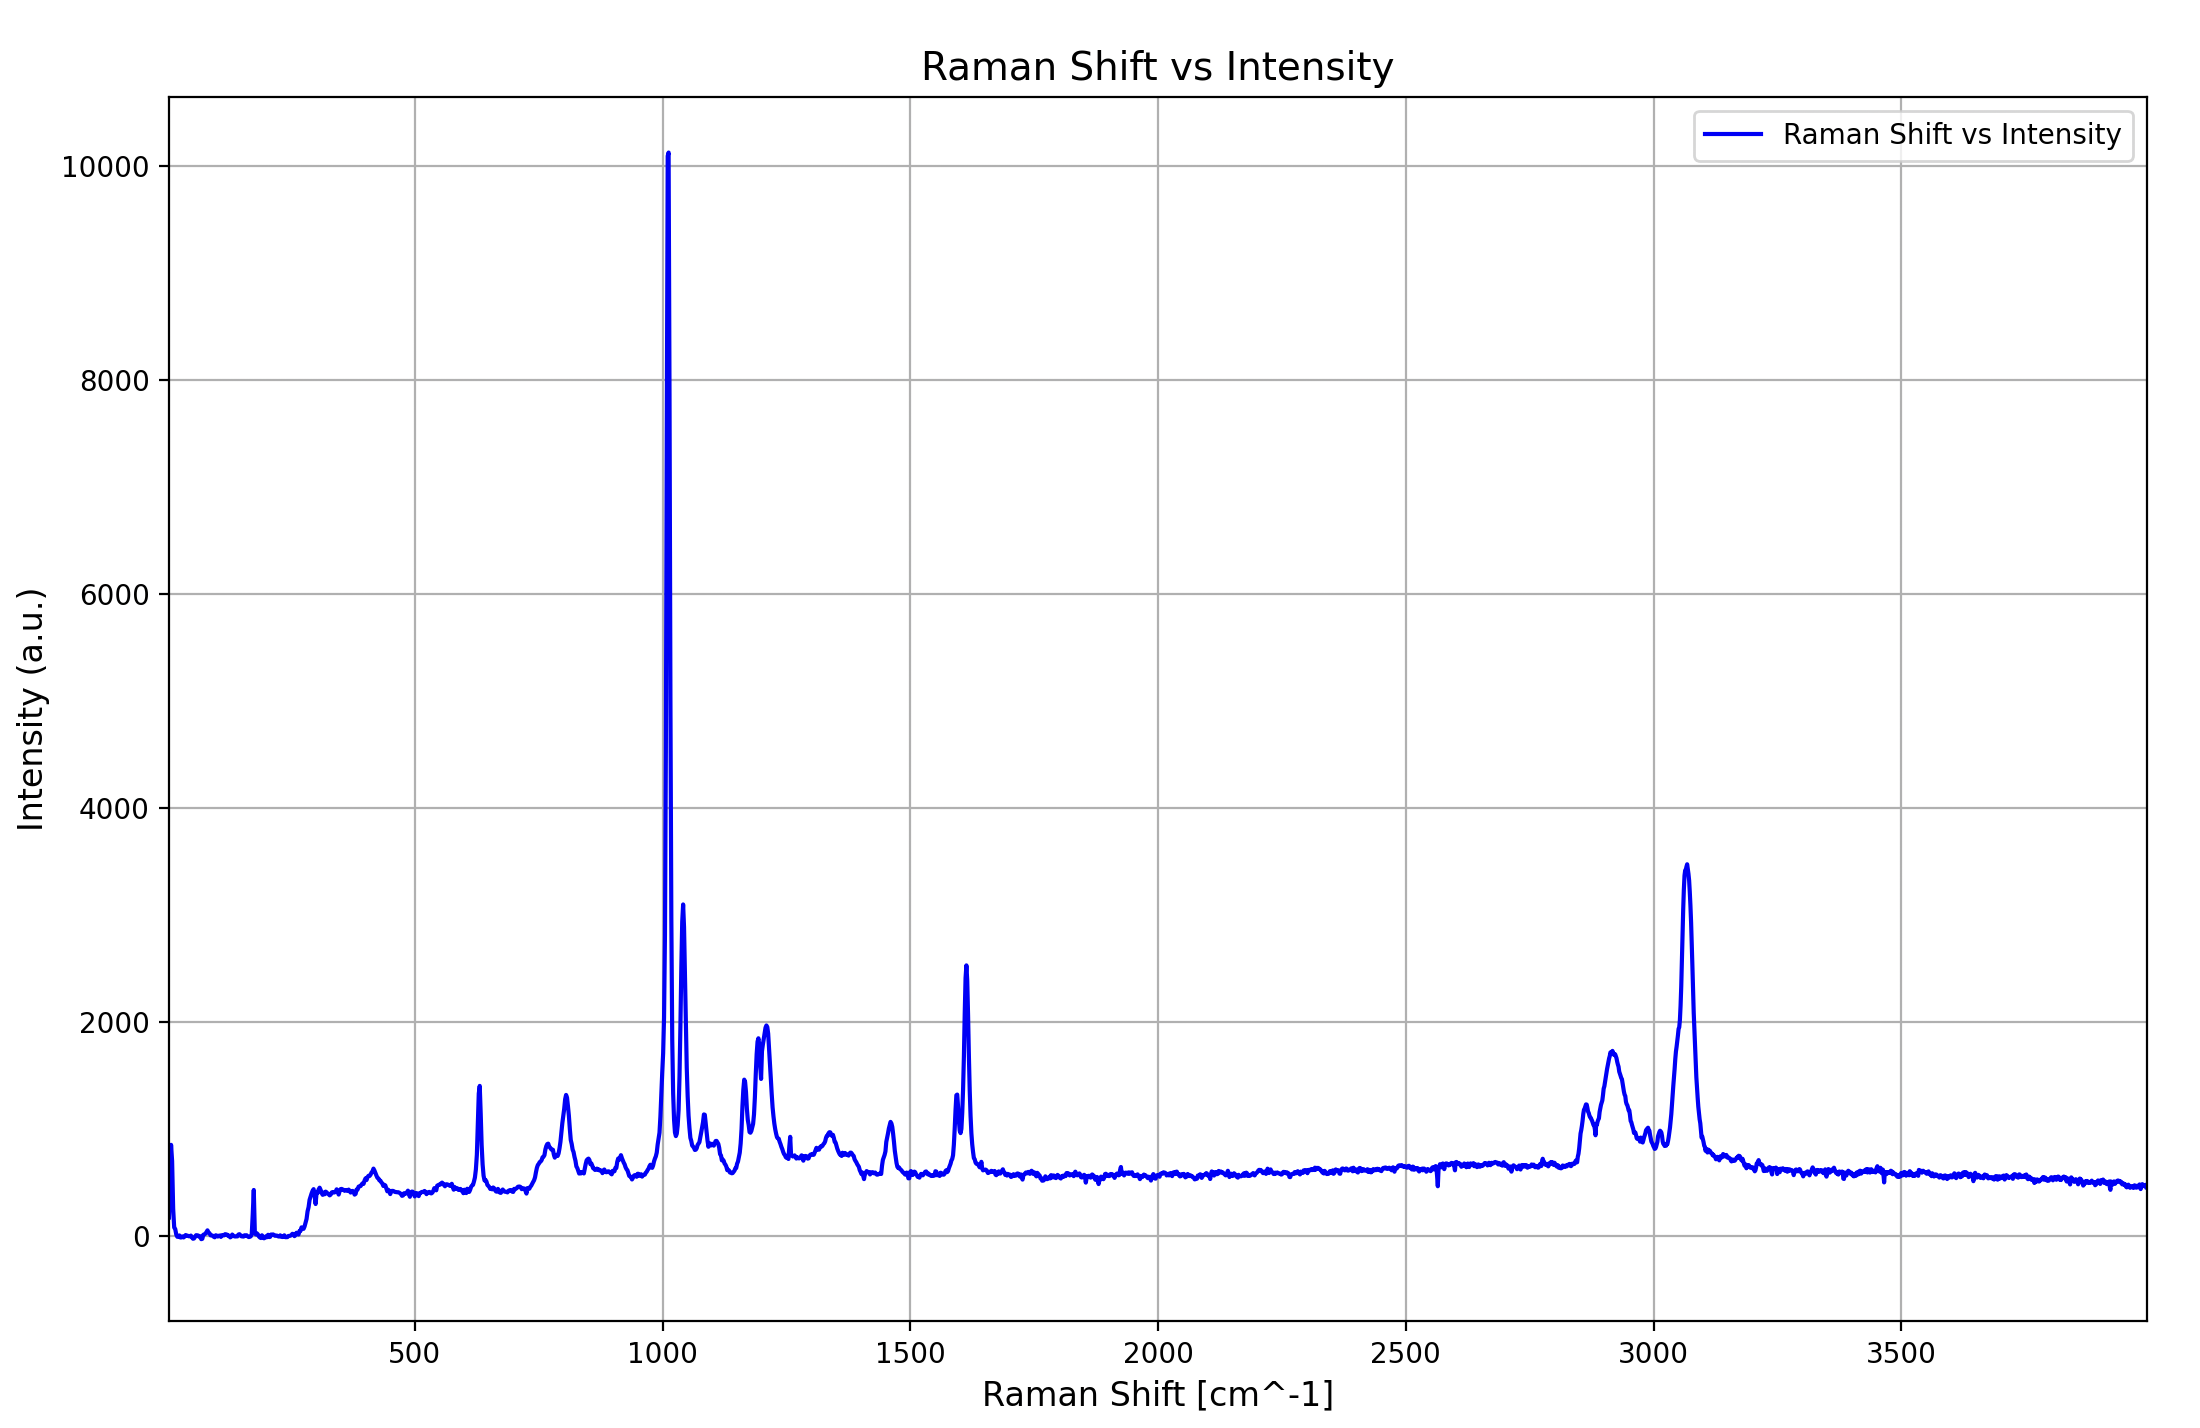
\includegraphics[width=1.2\textwidth]{images/raman_spectra/raman_shift_polystyreneh.png}}
        \caption{Experimental Raman spectrum of polystyrene}
        \label{fig:ps_x}
        \vspace{-10pt}
    \end{figure}

    \begin{figure}[h]
        \centering
        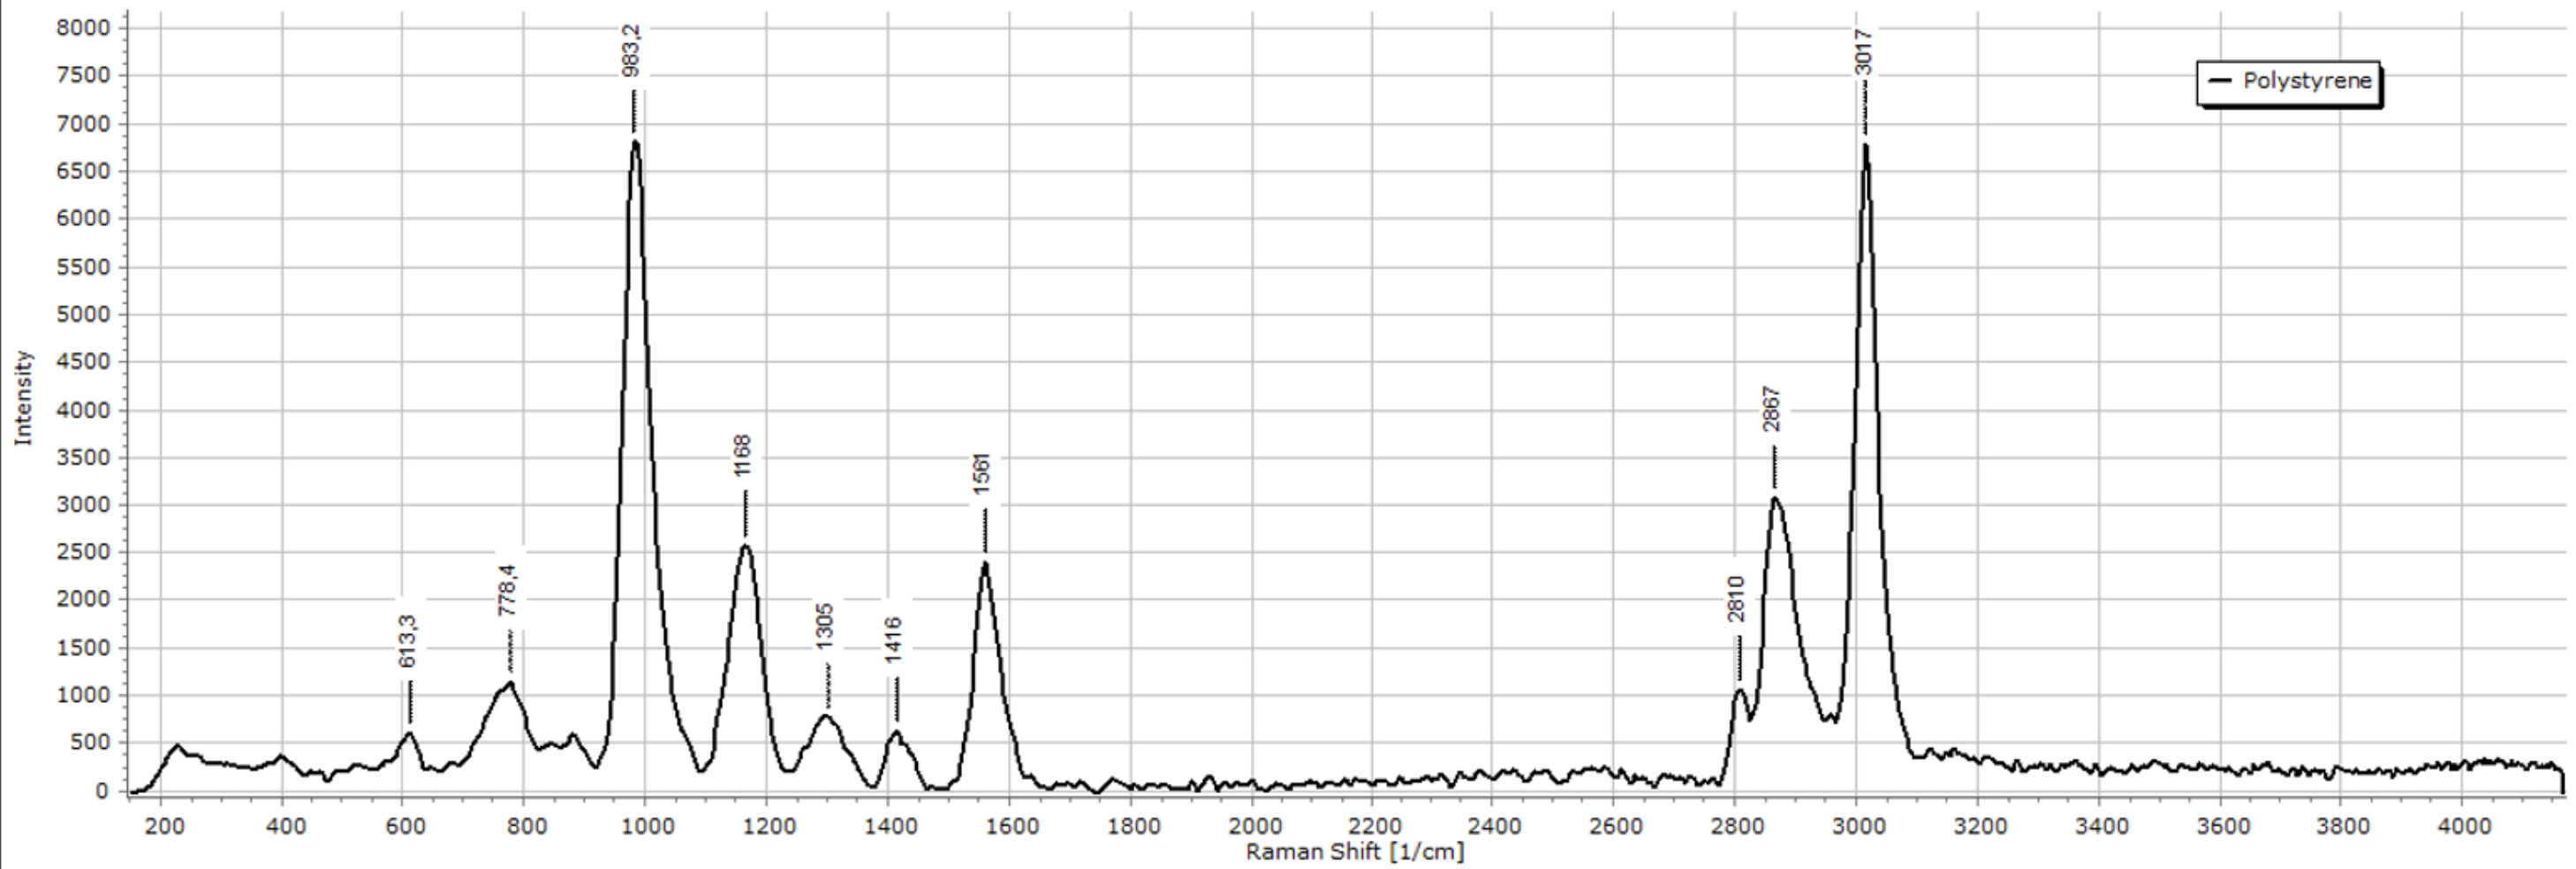
\includegraphics[width=\textwidth]{images/lit_raman/PS.png}
        \caption{Literature Raman spectrum of polystyrene \cite{spectrap}}
        \label{fig:ps_l}
    \end{figure}

\newpage

\section{Outlook}
The results of the conducted measurements show that Raman spectroscopy is in fact a viable option to identificate materials, specifically polymers, and a possible setup has been presented and tested. A qualitative explanation of the phenomenon has been provided.

\bigskip

One could continue to develop the setup in order to get cleaner data, ensuring less background noise and longer integration times, which was not possible due to limits given by the laser sensitivity. Raman spectroscopy could also be used in combination with IR-Spectroscopy to get more complete data.

\bigskip

As mentioned before, Raman spectroscopy is becoming more and more relevant in biochemical, medicinal and environmental sciences as a non-invasive method of identification. In connection to cancer research it is becoming more and more relevant since it can be used to not only identify specific molecules but also differenet tissue types. The identification of organic polymers, such as different plastics, is very relevant and constantly being developed in environmental science to identify mircoplastics.


\newpage

\section*{Literature List}
\printbibliography

\newpage

\section{Appendix}
The code used for the visualisation of the Raman spectra was written in python using the Sublime Text software on the 26th of November 2024.
\\


\begin{figure}[h]
    \centering
    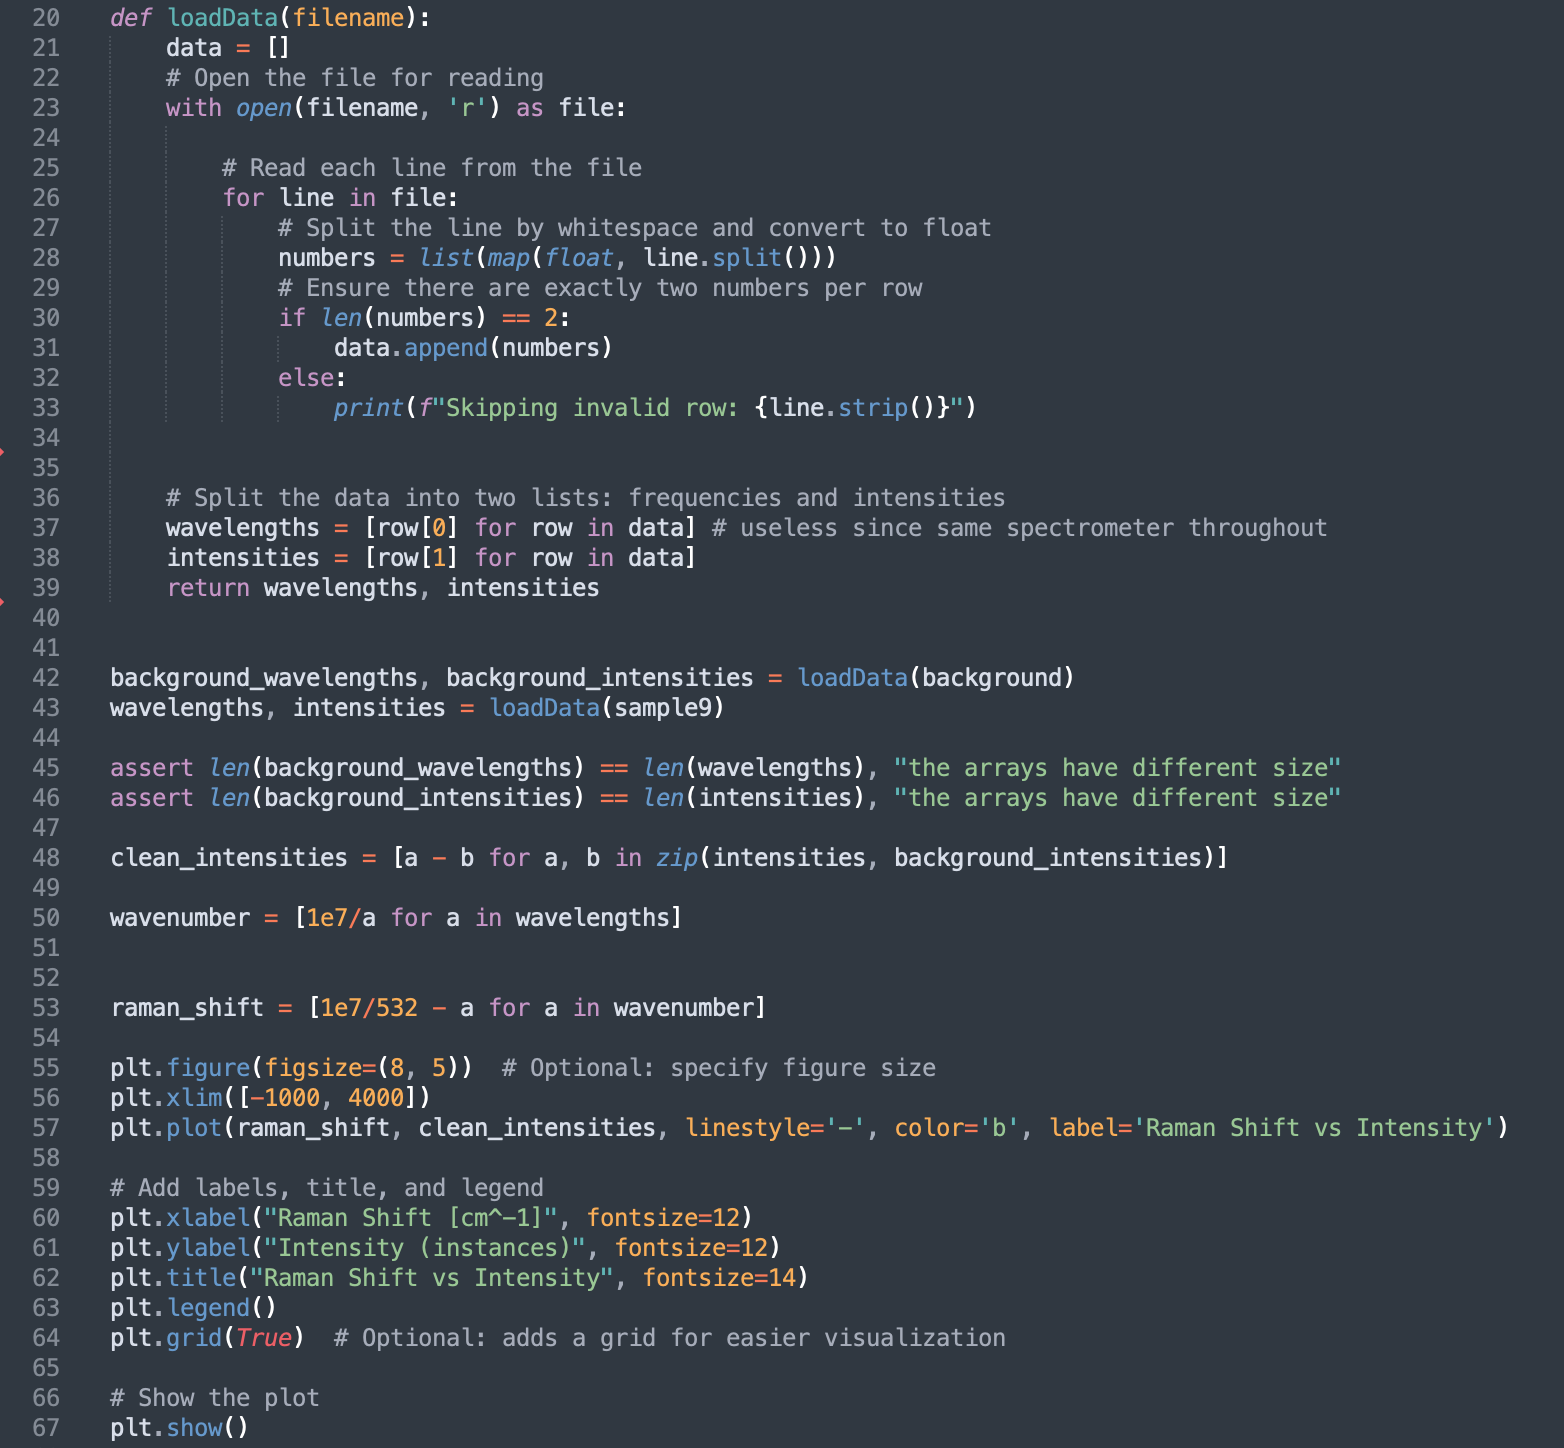
\includegraphics[width=0.9\textwidth]{images/code_raman_shift.png}
    \caption{Python code written for the calculation and visualisation of Raman shift}
    \label{fig:python}
\end{figure}

\newpage

\subsection*{Eigenständigkeitserklärung}

Der/die Unterzeichnete bestätigt mit Unterschrift, dass die Arbeit selbständig verfasst und in schriftliche Form gebracht worden ist, dass sich die Mitwirkung anderer Personen auf Beratung und Korrekturlesen beschränkt hat und dass alle verwendeten Unterlagen und Gewährspersonen aufgeführt sind.
\end{document}
